\documentclass{article}
\usepackage{amsmath}
\usepackage{amsfonts}
\usepackage{amssymb}

\newcommand{\mse}{\operatorname{mse}}
\newcommand{\bias}{\operatorname{bias}}
\newcommand{\se}{\operatorname{se}}
\newcommand{\Bernoulli}{\operatorname{Bernoulli}}
\newcommand{\Bin}{\operatorname{Bin}}
\newcommand{\Poisson}{\operatorname{Poisson}}
\newcommand{\Exp}{\operatorname{Exp}}
\newcommand{\MLE}{\operatorname{MLE}}


\usepackage{enumitem}

\usepackage{graphicx}

\usepackage{subcaption}

\usepackage{minted}

\usepackage{hyperref}

\begin{document}

\tableofcontents

\newpage

\section{Probability}
\subsection{Probability}
\begin{enumerate}
	\item Fill in the details of the proof of Theorem 1.8. Also, prove the monotone decreasing case.
		\begin{itemize}
			\item For the readers' convenience we restate the Continuity of Probabilities theorem. If $A_n \rightarrow A$ then $P(A_n) \rightarrow P(A)$ as $n \rightarrow \infty$. Here $A_n \rightarrow A_n$ means that either $A_n$ is monotone increasing ($A_n \subseteq A_{n + 1}$) and we define $A = \bigcup_{n = 1}^\infty A_n$, or, $A_n$ is monotone decreasing ($A_n \supseteq A_{n + 1}$) and we define $A = \bigcap_{n = 1}^\infty A_n$.
			\item We fill in the details now. First of all we want to show that $B_i \cap B_j = \emptyset$ for all $i \neq j$. Suppose without loss of generality that $i < j$ and note that $B_i \subseteq A_i$ then
			$$
			B_j = A_j \backslash \bigcup_{k = 1}^{j - 1} A_k
			$$
			and $B_i \subseteq A_i \subseteq \bigcup_{k = 1}^{j - 1}$ as such $B_i \cap B_j = \emptyset$.
			\item To see that $A_n = \bigcup_{i = 1}^n B_i$ let $x \in A_n$ then there exists a minimal $k = k(x)$ such that $x \in A_k$, i.e., for all $k' < k : x \notin A_{k'}$. Then $x \notin \bigcup_{i = 1}^{k - 1} A_i$ and therefore $x \in B_k$. Because $x$ are arbitrary it folows that $A_n \subseteq \bigcup_{i = 1}^n B_i$. On the other hand
			$$
			\bigcup_{i = 1}^n \underbrace{B_i}_{\subseteq\ A_i} \subseteq \bigcup_{i = 1}^n A_i = A_n,
			$$
			where we have used that $A_n$ is monotone increasing. The property that
			$$
			\bigcup_{i = 1}^\infty A_i = \bigcup_{i = 1}^\infty B_i
			$$
			holds is identical to the finite case, an element is part of the (countably) infinite union if there exists some minimual $i$ such that ...
			\item For the monotone decreasing case we instead want to define
			$$
			B_n := A_n \backslash \bigcup_{i > n} A_i.
			$$
		\end{itemize}
	\item Prove the statements in equation (1.1).
		\begin{itemize}
			\item This can immediately be seen by noting that $A \cup B = (A \backslash B) \cup (A \cap B) \cup (B \backslash A)$ is a disjoint union.
		\end{itemize}
	\item Let $\Omega$ be a sample space and let $A_1, A_2, \dots, $ be events. Define $B_n = \bigcup_{i = n}^\infty A_i$ and $C_n = \bigcap_{i = n}^\infty A_i$
		\begin{enumerate}
			\item Show that $(B_i)$ is monotone decreasing and that $(C_i)$ is monotone increasing.
			\item Show that $\omega \in \bigcap_{n = 1}^\infty B_n$ if and only if $\omega$ belongs to an infinite number of events $A_1, A_2, \dots$.
				\begin{itemize}
					\item Let $\omega \in \bigcap_{n = 1}^\infty B_n$ be such that $\omega$ does not belong to an infinite number of events $A_1, A_2, \dots$, i.e., there exists $N \in \mathbb{N}$ such that for all $k > N$ it follows that $\omega \notin A_k$. But then $\omega \notin B_k$ for all $k > N$ and as such does not lie in the intersection over all the $B_k$, which is a contradiction.
					\item Suppose $\omega$ lies in infinitely many $A_1, A_2, ...$. Then there exists a sequence $(A_{n_i})_{i \in \mathbb{N}}$ such that $n_i < n_{j}$ for all $i < j$ and such that $\omega \in A_{n_i}$ for all $i \in \mathbb{N}$. In that case
					$$
					\omega \in B_{n_i}
					$$
					for all $i \in \mathbb{N}$, in particular $\omega \in \cap_{i = \mathbb{N}} B_{n_i}$. Because $B_n$ is monotone decreasing the statement follows.
				\end{itemize}
			\item Show that $\omega \in \bigcup_{n = 1}^\infty C_n$ if and only if $\omega$ belongs to all the events $A_1, A_2, \dots$ except possibly a finite number of those events.
				\begin{itemize}
					\item Let $\omega \in \bigcup_{n = 1}^\infty B_n$ then there exists $n \geq 1$ such that $\omega \in B_n$. This means that $\omega \in \bigcap_{i = n}^\infty$, i.e., $\omega$ belongs to all $A_i$ where $i \geq n$.
					\item Now suppose $\omega$ belongs to all events $A_1, A_2, \dots$ except for a finite number of events. In that case there exist $N \in \mathbb{N}$ such that $\forall k \geq N : \omega \in A_k$. This means that
					$$
					\omega \in \bigcap_{i \geq k} A_i,
					$$
					i.e., $\omega \in C_k$. In particular this shows
					$$
					\omega \in C_k \subseteq \bigcup_{r \geq 1} C_r.
					$$
				\end{itemize}
		\end{enumerate}
	\item Let $\{A_i : i \in I\}$ be a collection of events where $I$ is an arbitrary index set. Show that
	$$
	\begin{aligned}
	\left( \bigcup_{i \in I} A_i \right)^c = \bigcap_{i \in I} A_i^c, && \left( \bigcap_{i \in I} A_i \right)^c = \bigcup_{i \in I} A_i^c
	\end{aligned}
	$$
	holds.

	Hint: First prove this for $I = \{1, 2, \dots, n\}$.
		\begin{itemize}
			\item I guess they want us to show it using induction in the hint, I'll just do it directly.
			$$
			\begin{aligned}
			\bigcap_i A_i^c &= \{x : \forall i : x \notin A_i\} \\
			&= \left\{x : \neg \left( \exists i : x \in A_i \right)\right\} \\
			&= \{x : \exists i : x \in A_i\}^c = \left( \bigcup_{i \in I} A_i \right)^c
			\end{aligned}
			$$
			The other equality can be proven analogously.
		\end{itemize}
	\item Suppose we toss a fair coin until we get exactly two heads. Describe the sample space S. What is the probability that exactly k tosses are required?
	\item Let $\Omega = \{0, 1, \dots \}$. Prove that there does not exist a uniform distribution on $\Omega$ (i.e., if $P(A) = P(B)$ whenever $|A| = |B|$, then $P$ cannot satisfy the axioms of probability.)
		\begin{itemize}
			\item Note that $P(\{0\}) \neq 0$ because otherwise $P = 0$, which would mean $P$ is not a probability function. But then it follows for all $n \in \mathbb{N}$:
			$$
			\begin{aligned}
			P(\{0, \dots, n\}) &= P\left(\bigcup_{k = 0}^n \{k\} \right) \\
			&= \sum_{k = 0}^n P(\{k\}) \\
			&= (n + 1)P(\{0\}) \rightarrow \infty
			\end{aligned}
			$$
			for $n \rightarrow \infty$, which is a contradiction to $P(\Omega) = +1$.
		\end{itemize}
	\item Let $A_1, A_2, \dots$ be events. Show that
	$$
	\left( \bigcup_{n = 1}^\infty A_n \right) \leq \sum_{n = 1}^\infty P(A_n).
	$$
	Hint: Define $B_n = A_n \backslash \bigcup_{i = 1}^{n - 1} A_i$. Then show that the $B_n$ are disjoint and that
	$$
	\bigcup_{n = 1}^\infty A_n = \bigcup_{n = 1}^\infty B_n.
	$$
	\begin{itemize}
		\item This was basically already shown in the first exercise, the only thing we mention here is that we only have to consider the case where the series on the right hand side converges, because the left hand side is always $\leq 1$.
	\end{itemize}
	\item Suppose that $P(A_i) = 1$ for each $i$. Prove that
	$$
	P\left( \bigcap_{i = 1}^\infty A_i \right) = 1.
	$$
		\begin{itemize}
			\item Note that $P(A_i^c) = 1 - P(A_i) = 0$ and that
			$$
			P\left( \bigcap_{i = 1}^\infty A_i \right) = 1 - P\left( \bigcup_{i = 1}^\infty A_i^c \right).
			$$
			The latter can be calculated as follows:
			$$
			\begin{aligned}
			0 &\leq P\left( \bigcup_{i = 1}^\infty A_i^c \right) \\
			&\leq \sum_{i = 1}^\infty P(A_i^c) = 0
			\end{aligned}
			$$
			where we have used that probability measures are subadditive. As such $P\left( \bigcup_{i = 1}^\infty A_i^c \right) = 0$ and therefore
			$$
			P\left( \bigcap_{i = 1}^\infty A_i \right) = 1.
			$$
		\end{itemize}
	\item For fixed $B$ such that $P(B) > 0$, show that $P(\cdot|B)$ satisfies the axioms of probability.
		\begin{itemize}
			\item[Axiom 1:] Let $A$ be arbitrary then
			$$
			P(A|B) = \frac{P(A, B)}{P(B)} \geq P(A, B) \geq 0.
			$$
			\item[Axiom 2:] $$P(\Omega|B) = \frac{P(\Omega, B)}{P(B)} = \frac{P(B)}{P(B)} = 1.$$
			\item[Axiom 3:]
			$$
			\begin{aligned}
			P\left(\left.\bigcup_{i = 1}^\infty A_i \right| B\right) &= \frac{1}{P(B)} P\left(\bigcup_{i = 1}^\infty A_i, \right) \\
			&= \frac{1}{P(B)} \sum_{i = 1}^\infty P(A_i, B) \\
			&= \sum_{i = 1}^\infty P(A_i|B).
			\end{aligned}
			$$
		\end{itemize}
	\item You have probably heard it before. Now you can solve it rigorously. It is called the "Monty Hall Problem." A prize is placed at random behind one of three doors. You pick a door. To be concrete, let's suppose you always pick door $1$. Now Monty Hall chooses one of the other two doors, opens it and shows you that it is empty. He then gives you the opportunity to keep your door or switch to the other unopened door.Should you stay or switch? Intuition suggests it doesn't matter. The correct answer is that you should switch. Prove it. It will help to specify he sample space and the relevant events carefully. Thus write $\Omega = \{(\omega_1, \omega_2): \omega_i \in \{1,2,3\}\}$ where $\omega_1$ is where the prize is and $\omega_2$ is the door Monty opens.
		\begin{itemize}
			\item Note that $\{(1, 1), (2, 2), (3, 3)\}$ are invalid because he'll never open the door with the price. The staying strategy wins on $\{(1, 2), (1, 3)\}$, the switching strategy wins on $\{(2, 3), (3, 2)\}$. Note that this means, if $\omega_1 \neq 1$, then we are guaranteed to win. As such we win whenever $\omega_1 \in \{2, 3\}$, as such the winning probability is $2/3$ for the switching strategy.
			\item This is a pretty subtle problem, the intuition is that him opening a door does not grant new information. If $\omega_1 = 1$ then his reveal is arbitrary and we lose on switching. If $\omega_1 = 2, 3$ then he's forced to reveal the nonempty door, as such either the remaining door is the price or $\omega_1 = 1$. As such when we switch we are guaranteed to win whenever $\omega_1 = 2, 3$.
		\end{itemize}
	\item Suppose that $A$ and $B$ are independent events. Show that $A^c$ and $B^c$ are independent events.
		\begin{itemize}
			\item
			$$
			\begin{aligned}
			P(A^c, B^c) &= P((A \cup B)^c) \\
			&= 1 - P(A \cup B) \\
			&= 1 - P(A) - P(B) + P(A, B) \\
			&= 1 - P(A) - P(B) + P(A)P(B) \\
			&= (1 - P(A))(1 - P(B)) \\
			&= P(A^c)P(B^C).
			\end{aligned}
			$$
		\end{itemize}
	\item There are three cards. The first is green on both sides, the second is red on both sides and the third is green on one side and red on the other. We choose a card at random and we see one side (also chosen at random) . If the side we see is green, what is the probability that the other side is also green? Many people intuitively answer $\frac{1}{2}$. Show that the correct answer is $\frac{2}{3}$.
	\item Suppose that a fair coin is tossed repeatedly until both a head and tail have appeared at least once.
		\begin{enumerate}
			\item Describe the sample space $\Omega$.
			\item What is the probability that three tosses will be required?
		\end{enumerate}
	\item Show that if $P(A) = 0$ or $p(A) = 1$ then $A$ is independent of every other event. Show that if A is independent of itself then $P(A)$ is either $0$ or $1$.
		\begin{itemize}
			\item $P(A) = P(A, A) = P(A)P(A) = P(A)^2 \iff P(A)(P(A) - 1).$
		\end{itemize}
	\item The probability that a child has blue eyes is $1 / 4$. assume independence between children. Consider a family with $3$ children.
		\begin{enumerate}
			\item If it is known that at least one child has blue eyes, what ist he probability that at least two children have blue eyes?
				\begin{itemize}
					\item Assuming that having blue eyes is independent from the other children then the chance that none of the siblings have blue eyes is $\left(\frac{3}{4}\right)^2 = \frac{9}{16}$. As such the probability is $7 / 16$. 
				\end{itemize}
			\item If it is known that the youngest child has blue eyes, what is the probability that at least two children have blue eyes?
				\begin{itemize}
					\item While this doesn't seem intuitive this actually changes the probabilities. To see this note that in the first problem the arrangements of having at least 2 blue eyed children were $BBB$, $BBG$, $BGB$, $GBB$ where the children are ordered by age. But now we disregard the case $GBB$ as such the probability becomes smaller.
					\item The probability is then $\left(\frac{1}{4}\right)^2 + \frac{1}{4} \frac{3}{4} + \frac{3}{4}\frac{1}{4}$
				\end{itemize}
		\end{enumerate}
	\item Prove Lemma 1.14.
		\begin{itemize}
			\item
			$$
			P(A|B) = \frac{P(A, B)}{P(B)} = \frac{P(A)P(B))}{P(B)} = P(A).
			$$
			\item
			$$
			\begin{aligned}
			P(AB) &= P(A, B) \frac{P(B)}{P(B)} \\
			&= P(A|B) P(B) \\
			& = P(B|A) \frac{P(A)}{P(B)} P(B) \\
			&= P(B|A)P(A).
			\end{aligned}
			$$
		\end{itemize}
	\item Show that
	$$
	P(A, B, C) = P(A|BC)P(B|C)P(C).
	$$
		\begin{itemize}
			\item
			$$
			P(ABC) = P(A|BC)P(BC) = P(A|BC)P(B|C)P(C).
			$$
		\end{itemize}
	\item Suppose $k$ events form a partition of the sample space $\Omega$, i.e., they are disjoint and 
	$$
	\bigcup_{i = 1}^k A_i = \Omega.
	$$
	Assume that $P(B) > O$. Prove that if $P(A_1|B) < P(A_1)$ then $P(A_i|B) > P(A_i)$ for some $i = 2, \dots, k$.
		\begin{itemize}
			\item Suppose this statement is wrong, i.e. $P(A_1|B) < P(A_1)$ and for all $i = 2, \dots, k$ we have $P(A_i|B) \leq P(A_i)$. It then follows that
			$$
			\begin{aligned}
			\sum_{i = 1}^k P(A_i|B) &= \underbrace{P(A_1|B)}_{< P(A_1)} + \sum_{i = 2}^k \underbrace{P(A_i|B)}_{\leq P(A_i)} \\
			&< P(A_1) + \sum_{i = 1}^k P(A_i) = 1.
			\end{aligned}
			$$
			Multiplying $\sum_{i = 1}^n P(A_i|B) < 1$ by $P(B) > 0$ yields
			$$
			\sum_{i = 1}^n P(A_i|B)P(B) < P(B).
			$$
			This is a contradiction because
			$$
			\begin{aligned}
			\sum_{i = 1}^n P(A_i|B)P(B) &= \sum_{i = 1}^n P(A_i, B) \\
			&= P\left(\bigcup_{i = 1}^n A_i , B\right) \\
			&= P(\Omega, B) = P(B).
			\end{aligned}
			$$
		\end{itemize}
	\item Suppose that $30\%$ of computer owners use a Macintosh, $50\%$ use Windows, and $20\%$ use Linux. Suppose that $65\%$ of the Mac users have succumbed to a computer virus, $82\%$ of the Windows users get the virus, and $50\%$ of the Linux users get the virus. We select a person at random and learn that her system was infected with the virus. What is the probability that she is a Windows user?
		\begin{itemize}
			\item Denote the operating systems by $M, W, L$ and having the virus by $V$. Using this notation we obtain $P(M) = 0.3$, $P(W) = 0.5$ and $P(L) = 0.2$. Furthermore $P(V|M) = 0.65$, $P(V|W) = 0.82$ and $P(V|L) = 0.5$ We can use the law of total probability to calculate the probability of a random person having a virus as being
			$$
			\begin{aligned}
			P(V) &= P(V, M) + P(V, W) + P(V, L) \\
			&= P(V|M)P(M) + P(V|W)P(W) + P(V|L)P(L) \\
			&= 0.65 \cdot 0.3 + 0.82 \cdot 0.5 + 0.5 \cdot 0.2 \\
			&= 0.705 = 70.5\%.
			\end{aligned}
			$$
			Now we can use Bayes' Theorem to calculate
			$$
			P(W|V) = P(V|W) \frac{P(W)}{P(V)} = 0.82 \frac{0.5}{0.705} = 0.5816 = 58.16\%
			$$
		\end{itemize}
	\item A box contains 5 coins and each has a different probability of showing heads. Let $P_1, P_2, P_3, P_4, P_5$ denote the probability of heads on each coin. Suppose that
	$$
	\begin{aligned}
	p_1 = 0,&& p_2 = 1/4,&& p_3 = 1/2,&& p_4 = 3/4,&& p_5 = 1.
	\end{aligned}
	$$
	Let $H$ denote "heads is obtained" and let $C_i$ denote the event that coin $i$ is selected.
	\begin{enumerate}
		\item Select a coin at random and toss it. Suppose a head is obtained. What is the posterior probability that coin $i$ was selected ($i = 1, ..., 5$)? In other words, find $P(C_i|H)$ for $i = 1, ..., 5$.
			\begin{itemize}
				\item Note that $P(C_i) = \frac{1}{5}$ and $P(H|C_i) = p_i$. The total probability of gettings heads is
				$$
				\begin{aligned}
				P(H) &= \sum_{i = 1}^5 P(H|C_i)P(C_i) \\
				&= \frac{1}{5} \sum_{i = 1}^5 P(H|C_i) \\
				&= \frac{1}{5} \sum_{i = 1}^5 p_i \\
				&= \frac{1}{5} (0 + 1/4 + 1/2 + 3/4 + 1) \\
				&= 0.5 = 50\%.
				\end{aligned}
				$$
				We can use Bayes' theorem to calculate
				$$
				\begin{aligned}
				P(C_i|H) &= P(H|C_i) \frac{P(C_i)}{P(H)} \\
				&= P(H|C_i) \frac{\frac{1}{5}}{0.5} \\
				&= P(H|C_i) \frac{2}{5}.
				\end{aligned}
				$$
				Using  this we obtain
				\begin{center}
				\begin{tabular}{|c|c|c|c|c|c|}
				\hline
				$i$ & 1 & 2 & 3 & 4 & 5 \\ 
				\hline
				$P(C_i|H)$ & 0 & 1/10 & 1/5 & 3/10 & 2/5 \\
				\hline
				\end{tabular}
				\end{center}
			\end{itemize}
		\item Toss the coin again. What is the probability of another head? In other words find $P(H_2|H_1)$ where $H_j$ = "heads on toss $j$."
			\begin{itemize}
				\item Suppose we have chosen the $ith$ coin then the probability of getting heads is $P(H|C_i)$. The probabilities of the individual coins have been calculated before and we just have to take the weighted sum over those.
\begin{minted}{python}
import numpy as np

mC = np.array([0, 1/10, 1/5, 3/10, 2/5])
mP = np.array([0, 0.25, 0.5, 0.75, 1])
np.dot(mC, mP)

> 0.75
\end{minted}
			\end{itemize}
		\item Find $P(C_i|B_4)$ where $B_4$ = "first head is obtained on toss $4$."
			\begin{itemize}
				\item First note that $P(C_i) = P(C_i, H_1) + P(C_i, H_1^c)$ as such
				$$
				\begin{aligned}
				P(C_i, H_1^c) &= P(C_i) - P(C_i, H_1) \\
				&= P(C_i) - P(C_i|H_1)P(H_1) \\
				&= \frac{1}{5} - P(C_i|H_1) \frac{1}{2}
				\end{aligned}
				$$
				as such
				\begin{center}
				\begin{tabular}{|c|c|c|c|c|c|}
				\hline
				$i$ & 1 & 2 & 3 & 4 & 5 \\ 
				\hline
				$P(C_i|H_i^c)$ & 0.2 & 0.15 & 0.1 & 0.05 & 0 \\
				\hline
				\end{tabular}
				\end{center}
				$P(H_1, H_2) = P(H_2|H_1)P(H_1) = \frac{3}{4}$
			\end{itemize}
	\end{enumerate}
	\item (Computer Experiment.) Suppose a coin has probability $p$ of falling heads up. If we flip the coin many times, we would expect the proportion of heads to be near $p$. We will make this formal later. Take $p = 0.3$ and $n = 1000$ and simulate $n$ coin flips. Plot the proportion of heads as a function of n. Repeat for $p = 0.03$.
		\begin{itemize}
			\item 
\begin{minted}{python}
import numpy as np
import matplotlib.pyplot as plt
import math

def Ex1_21(p = 0.3, n = 1000, draw = True, save = False):
    rand = np.random.random(size = 1000)
    _range = np.arange(1, n + 1)

    result = np.cumsum(rand < p) / _range

    fig, ax = plt.subplots()

    ax.plot(_range, result)

    if draw:
        plt.show()

    if save:
        # p = 0.213, n = 1000 -> 21pct_1000
        str_form = f"{math.floor(p * 100)}pct_{n}"
        fig.savefig(f"Ex1_21-{str_form}.png")

Ex1_21(p = 0.3, draw = True, save = True)
Ex1_21(p = 0.03, draw = True, save = True)
\end{minted}
		\begin{tabular}{cc}
			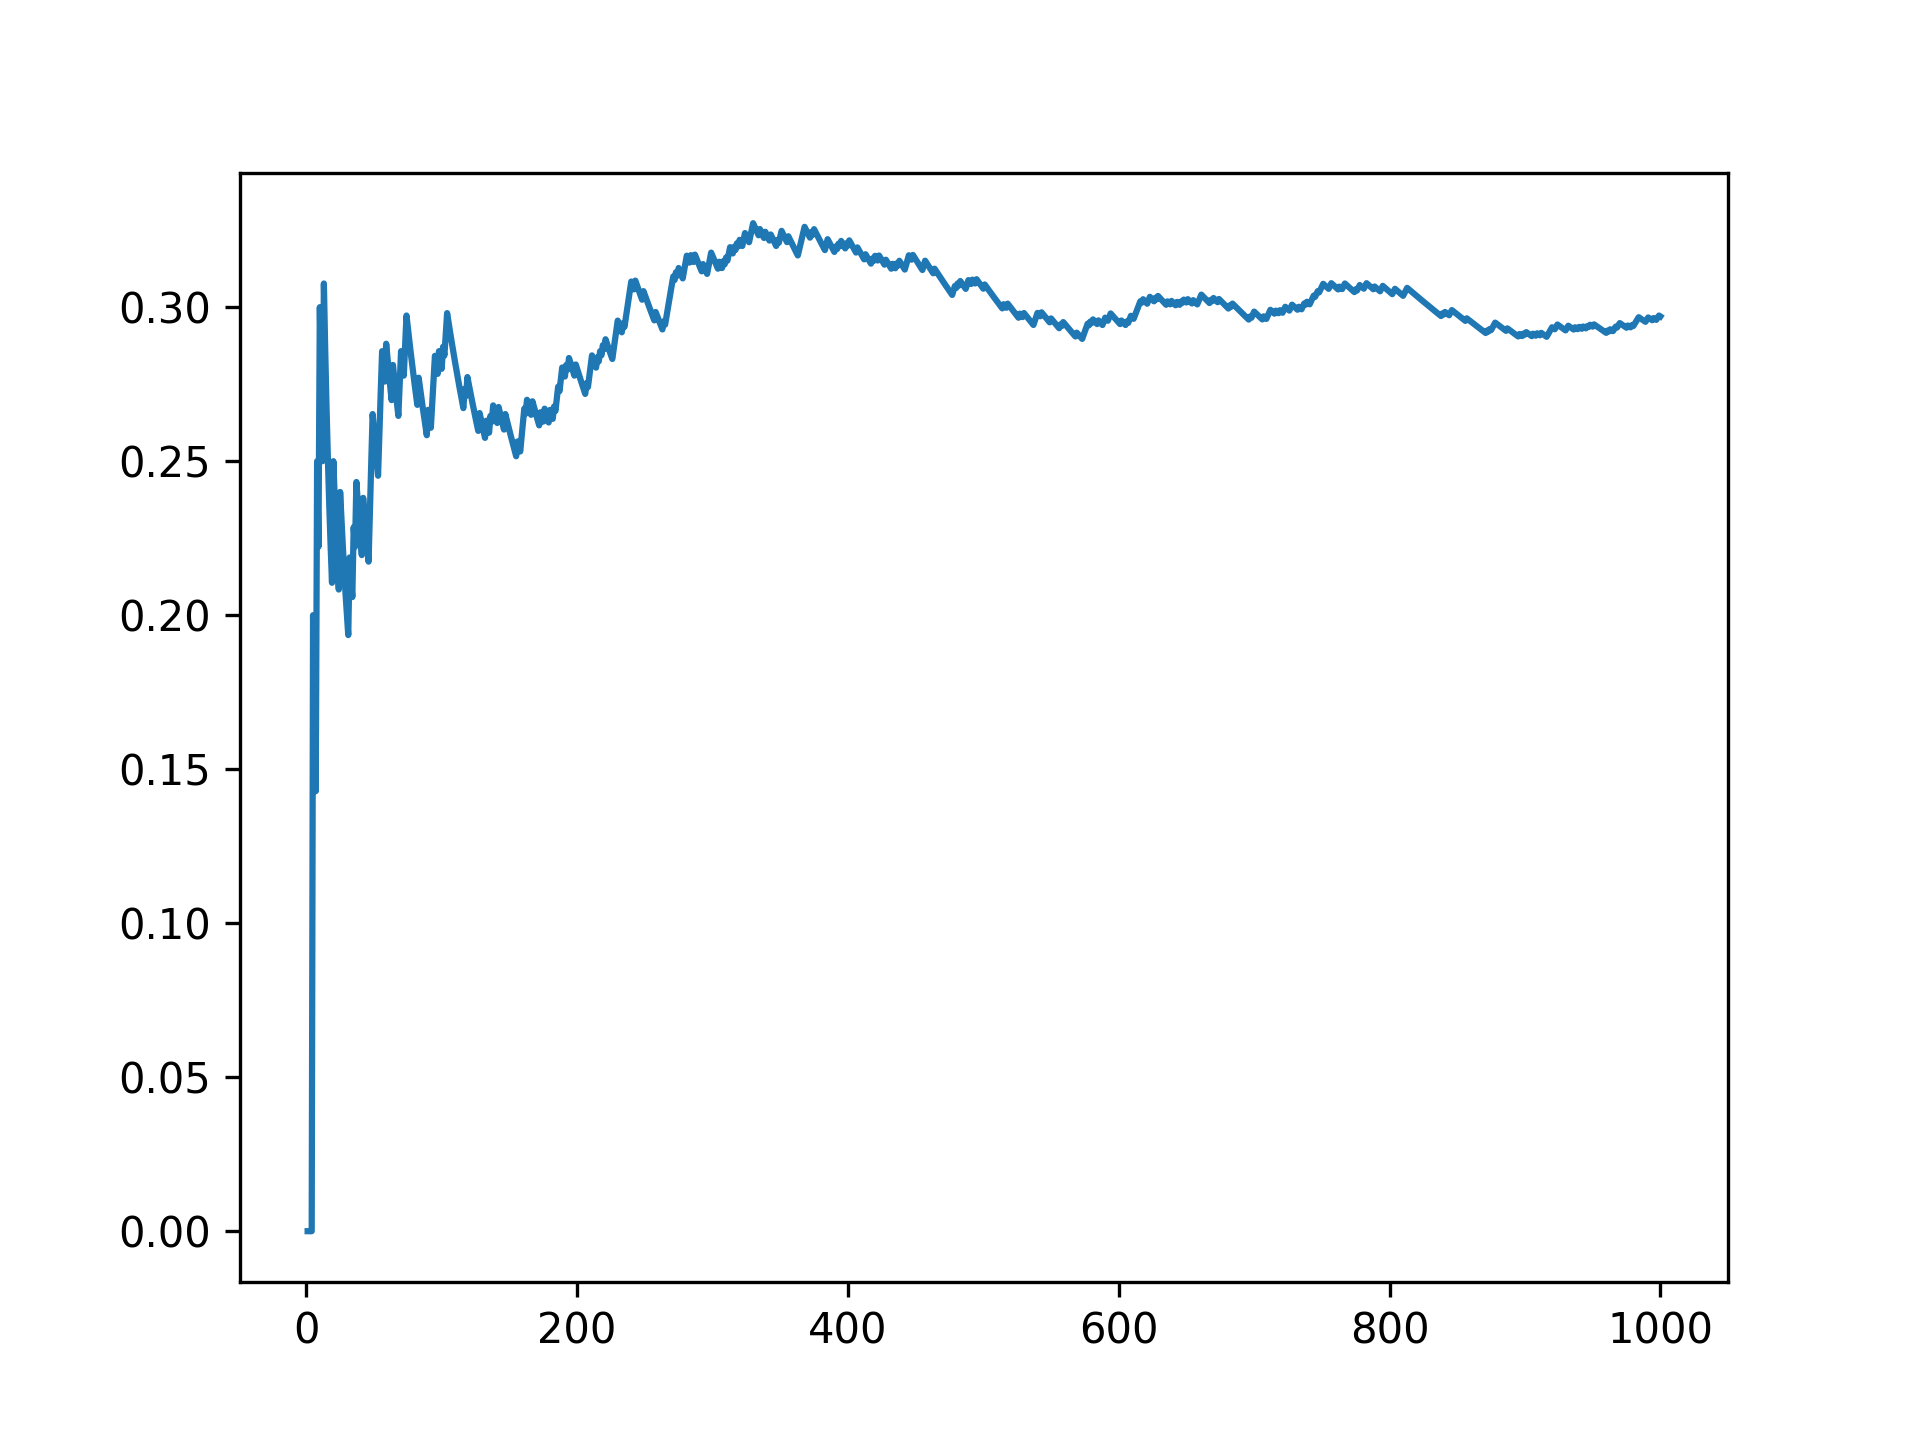
\includegraphics[width=0.45\textwidth]{1-Probability/Ex1_21-30pct_1000.png} &
			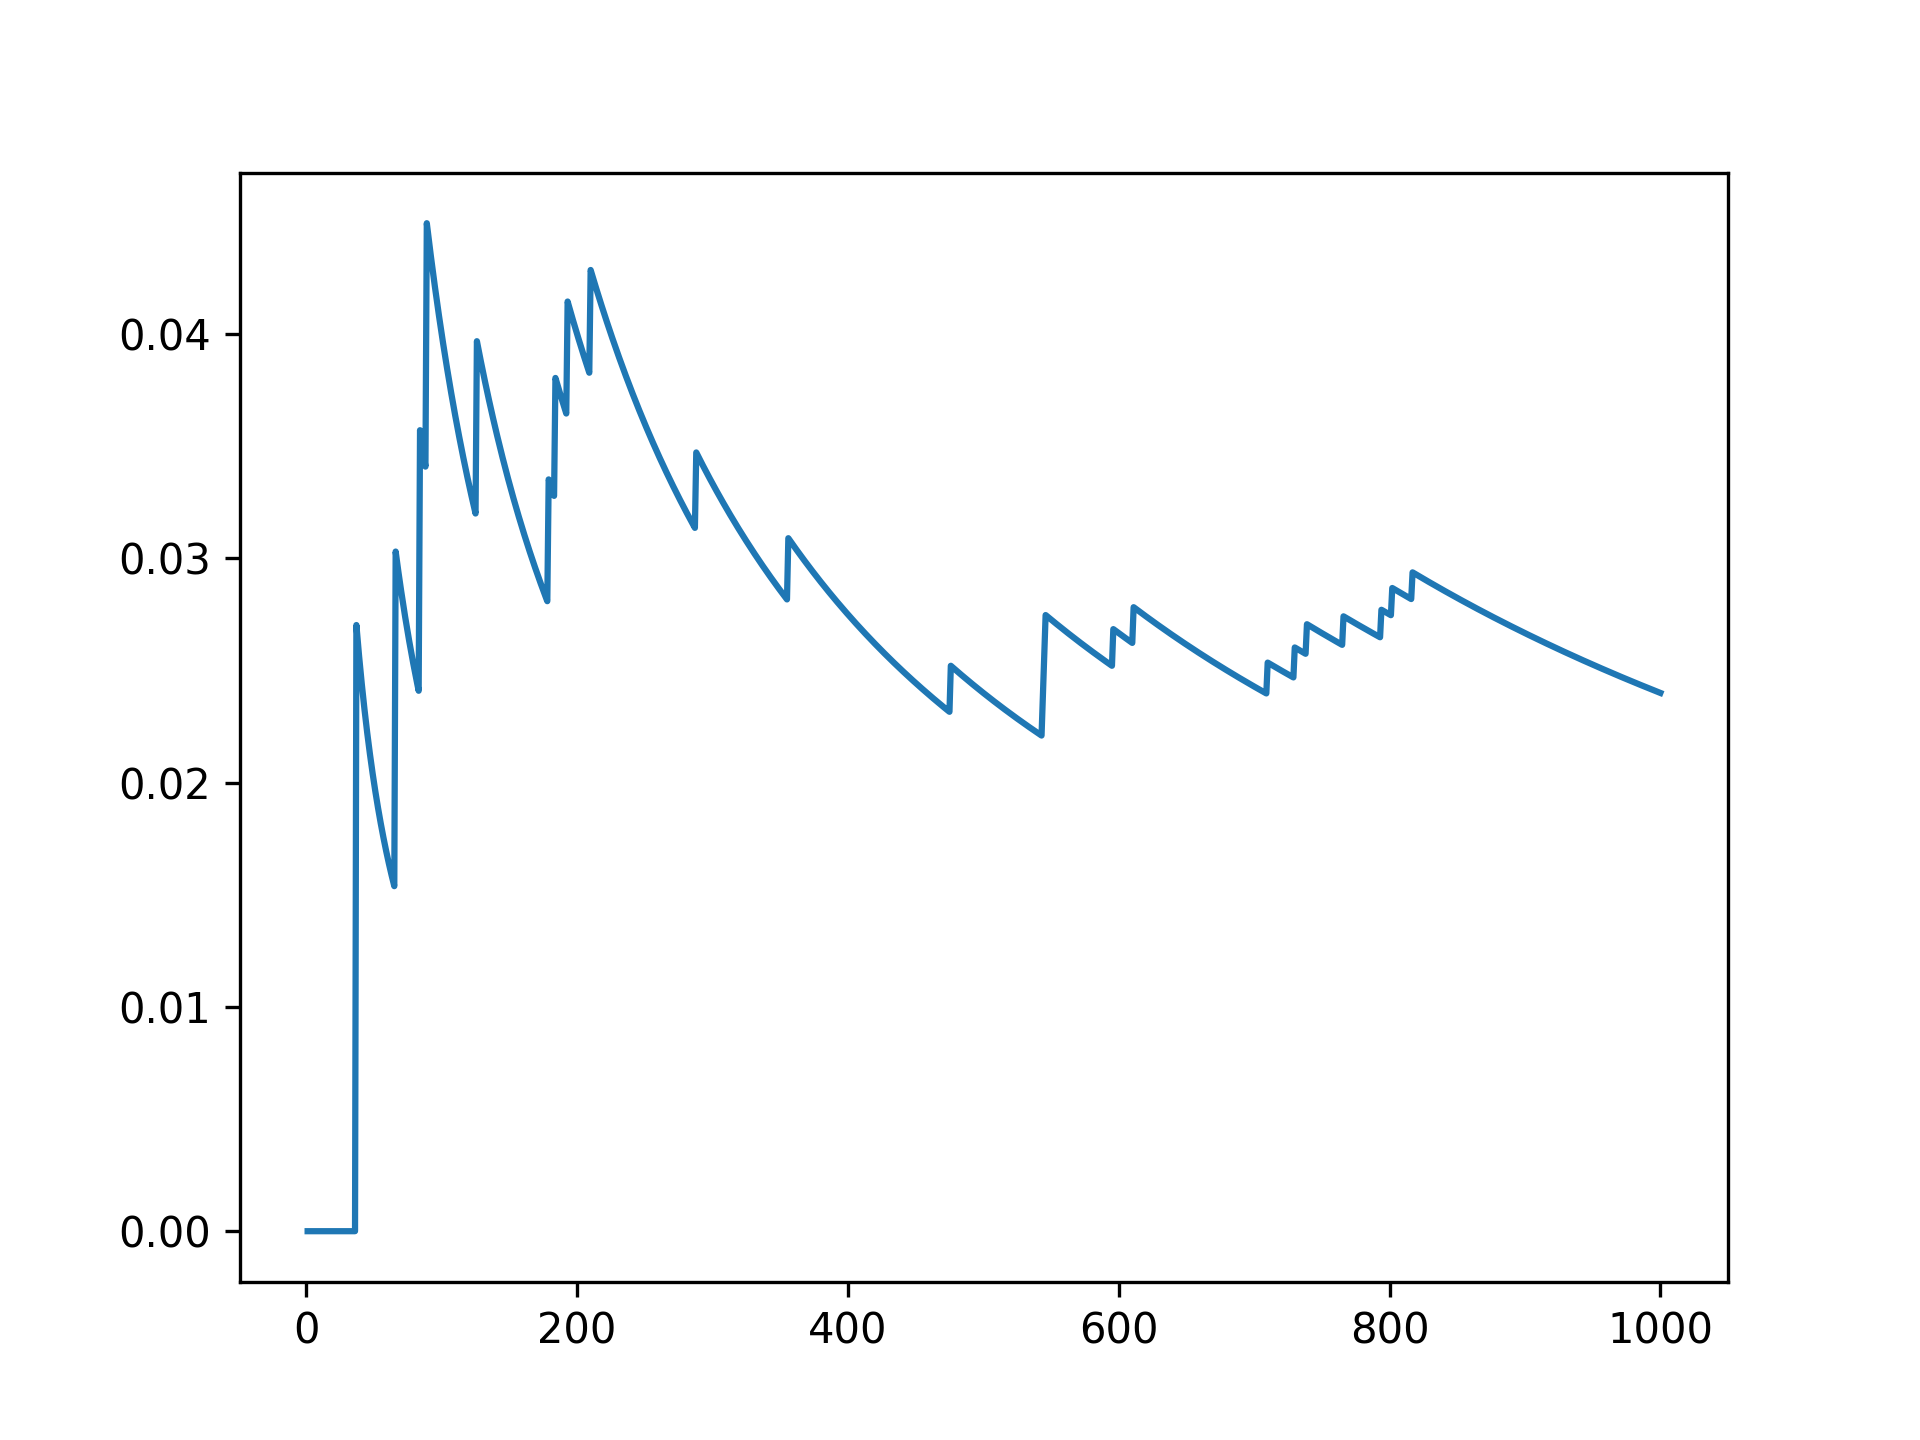
\includegraphics[width=0.45\textwidth]{1-Probability/Ex1_21-3pct_1000.png} \\
			(a) 30\% Probability & (b) 3\% Probability \\
		\end{tabular}
		\end{itemize}
	\item (Computer Experiment.) Suppose we flip a coin n times and let P denote the probability of heads. Let X be the number of heads. We call X a binomial random variable, which is discussed in the next chapter. Intuition suggests that X will be close to n p. To see if this is true, we can repeat this experiment many times and average the X values. Carry out a simulation and compare the average of the X's to n p . Try this for $p = 0.3$ and $n = 10$, $n = 100$, and $n = 1000$.
		\begin{itemize}
			\item 
\begin{minted}{python}
import numpy as np

def Ex1_22(p = 0.3, n = 1000, num_iter = 100):
    sum = 0
    for i in range(num_iter):
        rand = np.random.random(size = n)
        sum += np.sum(rand < p)

    mean = sum / num_iter
    expected = n * p
    delta = abs(mean - expected) / (expected)
    print(f"mean = {mean}, delta = {delta * 100:.2f}%")

for n in [10, 100, 1000]:
    Ex1_22(n = n)

> mean = 2.93, delta = 2.33%
> mean = 30.2, delta = 0.67%
> mean = 297.83, delta = 0.72%
\end{minted}
		\end{itemize}
	\item (Computer Experiment.) Here we will get some experience simulating conditional probabilities. Consider tossing a fair die. Let $A = \{2, 4, 6\}$ and $B = \{1, 2, 3, 4\}$. Then, $P(A) = 1/2$, $P(B) = 2/3$ and $P(AB) = 1/3$. Since $P(AB) = P(A)P(B)$, the events $A$ and $B$ are independent. Simulate draws from the sample space and verify that $\hat{P}(AB) = \hat{P}(A)\hat{P}(B)$ where $\hat{P}(A)$ is the proportion of times $A$ occurred in the simulation and similarly for $\hat{P}(AB)$ and $\hat{P}(B)$. Now find two events $A$ and $B$ that are not independent. Compute $\hat{P}(A)$,$\hat{P}(B)$ and $\hat{P}(AB)$. Compare the calculated values to their theoretical values. Report your results and interpret.
	\begin{itemize}
		\item
\begin{minted}{python}
import numpy as np

labels = ['P(A)', 'P(B)', 'P(A, B)', 'P(A)P(B)', 
          'P(A, B) - P(A)P(B)']
pct_str = lambda x : f"{x * 100:.2f}%"

def Ex1_23_helper(probabilities):
    for label, prob in zip(labels, probabilities):
        print(f"\t{label}: {pct_str(prob)}")

def Ex1_23(A, B, n = 10000):
    cap = A.intersection(B)

    # rand does [) so I need to increment high to get 6
    rand = np.random.randint(low = 1, high = 6 + 1, size = n)
    prob_A = sum(np.isin(rand, list(A))) / n
    prob_B = sum(np.isin(rand, list(B))) / n
    prob_cap = sum(np.isin(rand, list(cap))) / n

    prob_prod = prob_A * prob_B

    probabilities = [prob_A, prob_B, prob_cap, prob_prod,
                     prob_cap - prob_prod]

    print("Experimental Values")
    Ex1_23_helper(probabilities)

A, B = {2, 4, 6}, {1, 2, 3, 4}
print(f"A = {A}, B = {B}, AB = {A.intersection(B)}")
print("Theoretical Values")
Ex1_23_helper([1/2, 2/3, 1/3, 1/3, 0])
Ex1_23(A, B)
print()

A, B = {1, 2, 3}, {3, 4, 5, 6}
print(f"A = {A}, B = {B}, AB = {A.intersection(B)}")
print("Theoretical Values")
Ex1_23_helper([1/2, 2/3, 1/6, 1/3, -1/6])
Ex1_23(A, B)

> A = {2, 4, 6}, B = {1, 2, 3, 4}, AB = {2, 4}
> Theoretical Values
> 	P(A): 50.00%
> 	P(B): 66.67%
> 	P(A, B): 33.33%
> 	P(A)P(B): 33.33%
> 	P(A, B) - P(A)P(B): 0.00%
> Experimental Values
> 	P(A): 50.18%
> 	P(B): 67.42%
> 	P(A, B): 33.70%
> 	P(A)P(B): 33.83%
> 	P(A, B) - P(A)P(B): -0.13%
> 
> A = {1, 2, 3}, B = {3, 4, 5, 6}, AB = {3}
> Theoretical Values
> 	P(A): 50.00%
> 	P(B): 66.67%
> 	P(A, B): 16.67%
> 	P(A)P(B): 33.33%
> 	P(A, B) - P(A)P(B): -16.67%
> Experimental Values
> 	P(A): 50.20%
> 	P(B): 66.30%
> 	P(A, B): 16.50%
> 	P(A)P(B): 33.28%
> 	P(A, B) - P(A)P(B): -16.78%
\end{minted}
		\end{itemize}
\end{enumerate}

\subsection{Random Variables}
\begin{enumerate}
	\item Show that
	$$
	P(X = x) = F(x^+) - F(x^-).
	$$
		\begin{itemize}
			\item Note that $(\infty, x)$ and $\{x\}$ are disjoint as such
			$$
			P(X \leq x) = P(X < x) + P(X = x).
			$$
			This allows us to calculate:
			$$
			\begin{aligned}
			P(X = x) &= P(X \leq x) - P(X < x) \\
			&= F(x) - P(X < x) \\
			&= F(x) - \lim_{\varepsilon \searrow 0} P(X \leq x - \varepsilon) \\
			&= F(x) - \lim_{y \searrow x} P(X \leq y) \\
			&= F(x) - \lim_{y \searrow x} F(y) \\
			&= F(x^+) - F(x^-),
			\end{aligned}
			$$
			where we have used that $F(x) = F^+(x)$ by definition of CDFs.
		\end{itemize}
	\item Let $X$ be such that $P(X = 2) = P(X = 3) = 1 / 10$ and $P(X = 5) = 8 / 10$. Plot the CDF $F$. Use $F$ to find $P(2 < X \leq 4.8)$ and $P(2 \leq X \leq 4.8)$.
		\begin{itemize}
			\item
			\begin{minted}{python}
import numpy as np
import matplotlib.pyplot as plt

def Ex2_2(draw = True, save = False):
    x = np.arange(start=0, stop = 6, step = 0.2)
    F = (x >= 2) * 0.1 + (x >= 3) * 0.1 + (x >= 5) * 0.8
    plt.step(x, F, where='post')

    if save:
        plt.savefig("Ex2_2.png")
    if draw:
        plt.show()

    right = np.where(abs(x - 4.8) < 0.1)[0]
    left = np.where(abs(x - 2) < 0.1)[0]
    print("P(2 <  X <= 4.8) = ", (F[right] - F[left])[0])
    print("P(2 <= X <= 4.8) = ", (F[right] - F[left - 1])[0])

Ex2_2(draw = False, save = False)

> P(2 <  X <= 4.8) =  0.1
> P(2 <= X <= 4.8) =  0.2
			\end{minted}
			\begin{center}
				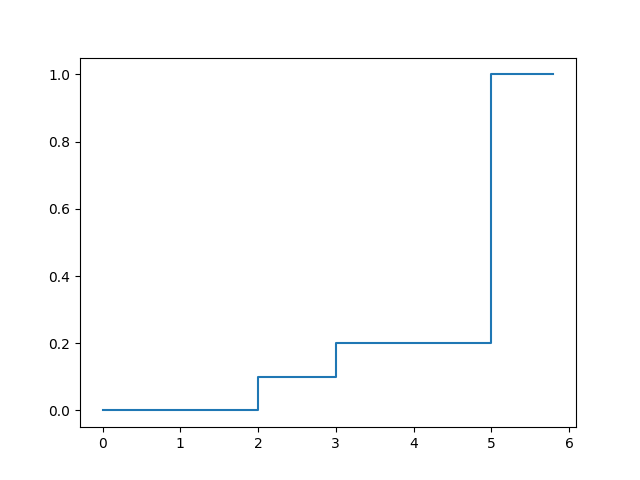
\includegraphics[width=\linewidth]{2-Random_Variables/Ex2_2.png}
			\end{center}
		\end{itemize}
	\item Prove Lemma 2.15.
		\begin{itemize}
			\item (1) was shown in the first exercise.
			\item Note that
			$$
			P(X \leq y) = P(x < X \leq y) + P(X \leq x),
			$$
			i.e.,
			$$
			P(x < X \leq y) = P(X \leq y) - P(X \leq x) = F(y) - F(y).
			$$
			\item
			$$
			P(X > c) = P((X \leq x)^c) = 1 - P(X \leq x) = 1 - F(x).
			$$
			\item If $X$ is continuous then it has a PDF, i.e., a function $f$ such that
			$$
			F(t) = \int_{-\infty}^t f(x) dx.
			$$
			The statements then follow from the fact that individual points don't change the integral.
		\end{itemize}
	\item Let $X$ have probability density function
	$$
		f(x) = 
	\begin{cases} 
	\frac{1}{4} & \text{if } 0 < x < 1 \\
	\frac{3}{8} & \text{if } 3 < x < 5 \\
	0 & \text{otherwise}
	\end{cases}
	$$
		\begin{enumerate}
			\item Find the cumulative distribution function of $X$.
				\begin{itemize}
					\item We can obtain the CDF $F$ of $f$ by integration:
					$$
					F(t) := \int_{-\infty}^t f(x) dx,
					$$
					For $t \leq 0$ we have $F(t) = 0$. Let $t \in (0, 1)$ then
					$$
					F(t) = \int_0^t \frac{1}{4} dx = \frac{t}{4}.
					$$
					For $t \in [1, 3]$ we have
					$$
					F(t) = \int_0^1 f(x) dx = \frac{1}{4}.
					$$
					Now let $t \in (3, 5)$ then
					$$
					\begin{aligned}
					F(t) &= \int_0^1 f(x) dx + \int_3^t f(x) dx \\
					&= \frac{1}{4} + (t - 3) \frac{3}{8}.
					\end{aligned}
					$$
					And for $t \geq 5 : F(t) = 1$. In total this shows that
					$$
					F(t) = 
					\begin{cases} 
					0, & \text{if } t \leq 0, \\
					\frac{t}{4}, & \text{if } t \in (0, 1), \\
					\frac{1}{4}, & \text{if } t \in [1, 3], \\
					\frac{1}{4} + \frac{3}{8}(t - 3), & \text{if } t \in (3, 5), \\
					1, & \text{if } t \geq 5.
					\end{cases}
					$$
				\end{itemize}
			\item Let $Y = 1 / X$. Find the probability density function $f_Y(y)$ for $Y$. Hint. Consider three cases: $\frac{1}{5} \leq y \leq \frac{1}{3}$, $\frac{1}{3} \leq y \leq 1$, and $y \geq 1$.
				\begin{itemize}
					\item First of all, note that $0 < X < 5$, as such $\frac{1}{5} < Y$. This means that
					$$
					P(Y \leq y) = P\left(\frac{1}{5} < Y \leq y \right)
					$$
					Now suppose $y \in \left(\frac{1}{5}, \frac{1}{3} \right)$, then
					$$
					P\left(Y \leq y\right) = P\left( \frac{1}{5} < Y \leq y \right)
					$$
					By definition
					$$
					\frac{1}{5} < Y \leq y \iff \frac{1}{y} \leq \frac{1}{Y} < 5 \iff \frac{1}{y} \leq X < 5.
					$$
					Then
					$$
					P\left(Y \leq y\right) = P\left(\frac{1}{y} \leq X < 5\right) = F(5) - F\left( \frac{1}{y} \right).
					$$
					This can then be computed by noting that $F(5) = 1$ and $F(1 / y) = \frac{1}{4} + \frac{3}{8}(\frac{1}{y} - 3)$.

					For $\frac{1}{3} \leq y \leq 1$ we have
					$$
					P\left(Y \leq y\right) = F(3) - F\left(\frac{1}{y}\right)
					$$
					and this is equal to $\frac{1}{4}$. For $y \geq 1$ we have $\frac{1}{y} \leq 1$ and
					$$
					\frac{1}{4} - \frac{1}{4y}.
					$$
					In total this means [TODO: Finish this].
				\end{itemize}
		\end{enumerate}
	\item Let $X$ and $Y$ be discrete random variables. Show that $X$ and $Y$ are independent if and only if $f_{X, Y}(x, y) = f_X(x)f_Y(y)$ for all $x$ and $y$.
	\item Let $X$ have distribution $F$ and density function $f$ and let $A$ be a subset of $\mathbb{R}$. Denote by $I_A(x)$ the indicator function for $A$. Let $Y = I_A(X)$. Find an expression for the cumulative distribution of $Y$. Hint: first find the probability mass function for $Y$.
		\begin{itemize}
			\item Denote the CDF of $Y$ by $G$. Note that $Y$ either takes $0$ or $1$ as its value. The PDF $g$ of $Y$ is $g(t) = 1$ if $X(t) \in A$ and $0$ else. This means that the CDF for $y < 0$ is just $0$, for $0 \leq y < 1$, $G(y) = P(X \in A)$ and $G(y) = 1$ for all $y \geq 1$. Note that
			$$
			P(X \notin A) = 1 - P(X \in A) = 1 - \int_A f(x) dx.
			$$
		\end{itemize}
	\item Let $X$ and $Y$ be independent and suppose that each has a $\operatorname{Uniform}(0, 1)$ distribution. Let $Z = \min\{X, Y\}$. Find the density $f_Z(z)$ for $Z$. Hint: It might be easier to first find $P(Z > z)$.
		\begin{itemize}
			\item By definition we have 
			$$
			P(Z > z) = P(\min{X, Y} > z) = P(X > z, Y > z),$$
			because $X$ and $Y$ are independent it follows that this is equal to $P(X > z)P(Y > z)$, because both of those have the same distribution those two probabilities are the same:
			$$
			P(X > z)P(Y > z) = P(X > z)^2 = (1 - P(X \leq z))^2 = (1 - z)^2.
			$$
			As such
			$$
			P(Z \leq z) = 1 - p(Z > z) = 1 - (1 - z)^2 = 2z - z^2.
			$$
			Differentiating this yields the PDF
			$$
			f_Z(z) = 2 - 2z.
			$$
		\end{itemize}
	\item Let $X$ have CDF $F$. Find the CDF of $X^+ = \max{0, X}$.
		\begin{itemize}
			\item Note that for $y \leq 0$ we have $P(X^+ \leq y) = F(0)$. For $x > 0$ we have
			$$
			\begin{aligned}
			F(X^+ \leq x) &= F(X^+ \leq 0) + P(0 < X^+ \leq x) \\
			&= F(0) + P(0 < X \leq x) \\
			&= F(0) + F(x) - F(0) \\
			&= F(x).
			\end{aligned}
			$$
		\end{itemize}
	\item Let $X \sim \operatorname{Exp}(\beta)$. Find $F(x)$ and $F^{-1}(q)$.
		\begin{itemize}
			\item The PDF of $f$ is given by $f(x) = \frac{1}{\beta} e^{- x / \beta}$ for $x > 0$ and $0$ for $x \leq 0$. We obtain the CDF of $X$ by integrating. For $t \leq 0$ we have F(t) and for $t > 0$
			$$
			F(t) = \int_{-\infty}^t f(x) dx = \int_0^t \frac{1}{\beta} e^{-x / \beta} dx.
			$$
			Recall that the antiderivative of $e^{Ax}$ is $\frac{1}{A} e^{Ax}$ as such
			$$
			\begin{aligned}
			F(t) &= \left. \frac{1}{\beta} \frac{1}{-\frac{1}{\beta}} e^{-x / \beta} \right|_{x = 0}^{x = t} \\
			&= - e^{-t / \beta} + e^{-0 / \beta}.
			\end{aligned}
			$$
			As such
			$$
			F(t) = 1 - e^{-t / \beta}.
			$$
			Per definition $F^{-1}(q) = \inf \{x : F(x) > q\}$ for $q \in [0, 1]$. For a continuous and monotone increasing function $F$ (which is the case for the exponential distribution) this is simply
			$$
			x = F^{-1}(q).
			$$
			As such we want to solve $F(x) = q$ for $x$, this is a straightforward computation:
			$$
			\begin{aligned}
			&& q &= 1 - e^{-x / \beta} \\
			\iff&& e^{-t / \beta} &= 1 - q \\
			\iff&& -t/\beta &= \log(1 - q) \\
			\iff&& t &= -\beta \log(1 - q).
			\end{aligned}
			$$
		\end{itemize}
	\item Let $X$ and $Y$ be independent. Show that $g(X)$ is independent of $h(Y)$ where $g$ and $h$ are functions.
	\item Suppose we toss a coin once and let $p$ be the probability of heads. Let $X$ denote the number of heads and let $Y$ denote the number of tails.
		\begin{enumerate}
			\item Prove that $X$ and $Y$ are dependent.
				\begin{itemize}
					\item Suppose $p \in (0, 1)$ then $P(X = 1) = p$ and $P(Y = 1) = 1 - p$ but $P(X = 1, Y = 1) = 0$, as such $X$ and $Y$ can't be independent.
				\end{itemize}
			\item Let $N \sim \operatorname{Poisson}(\lambda)$ and suppose we toss a coin $N$ times. Let $X$ and $Y$ be the number of heads and tails. Show that $X$ and $Y$ are independent.
		\end{enumerate}
	\item Prove Theorem 2.33: Suppose that the range of $X$ and $Y$ is a (possibly infinite) rectangle. If $f(x, y) = g(x)h(y)$ for some functions $g$ and $h$ (not necessarily probability density functions) then $X$ and $y$ are independent.
	\item Let $X \sim \mathcal{N}(0, 1)$ and let $Y = e^X$.
		\begin{enumerate}
			\item Find the PDF for $Y$. Plot it.
				\begin{itemize}
					\item Note that $P(Y \leq t) = P(e^X \leq t) = P(X \leq \log(t))$. We can obtain the PDF $g$ of $Y$ by differentiation:
					$$
					\frac{d}{dt} F(\log(t)) = \frac{1}{\sqrt{2\pi} t} e^{- \frac{\log(t)^2}{2}}.
					$$
					\begin{minted}{python}
import numpy as np
import matplotlib.pyplot as plt

x = np.arange(start = 0.01, stop = 7, step = 0.01)
y = np.exp(- np.log(x)**2 * 0.5) * 0.5 / x
y = y / np.sqrt(2 * np.pi)
plt.plot(x, y)

plt.savefig('Ex2_13a.png')
					\end{minted}
					\begin{center}
						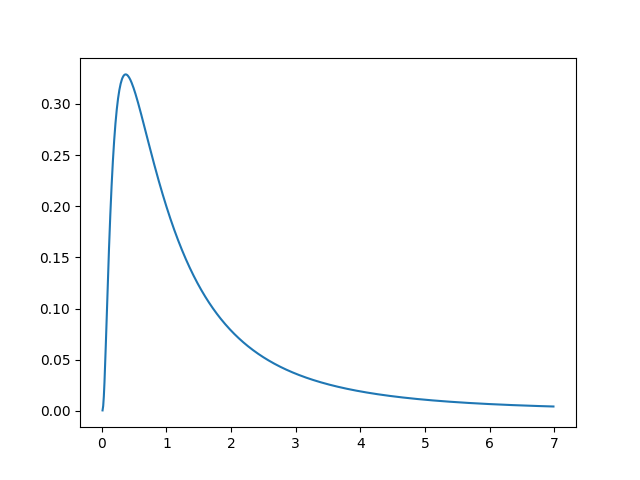
\includegraphics[width=\linewidth]{2-Random_Variables/Ex2_13a.png}
					\end{center}
				\end{itemize}
			\item (Computer Experiment) Generate a vector $x = (x_1, \dots, x_{10000})$ consisting of $10000$ random standard Normals. Let $y = (y_1, \dots, y_{10000})$ where $y_i = e^{x_i}$. Draw a histogram of $y$ and compare it to the PDF you found in part $(a)$.
				\begin{itemize}
					\item
					\begin{minted}{python}
import numpy as np
import matplotlib.pyplot as plt

x = np.random.randn(10000)
y = np.exp(x)

plt.hist(y, bins=50)
plt.savefig('Ex2_13b.png', dpi=300)
					\end{minted}
					\begin{center}
						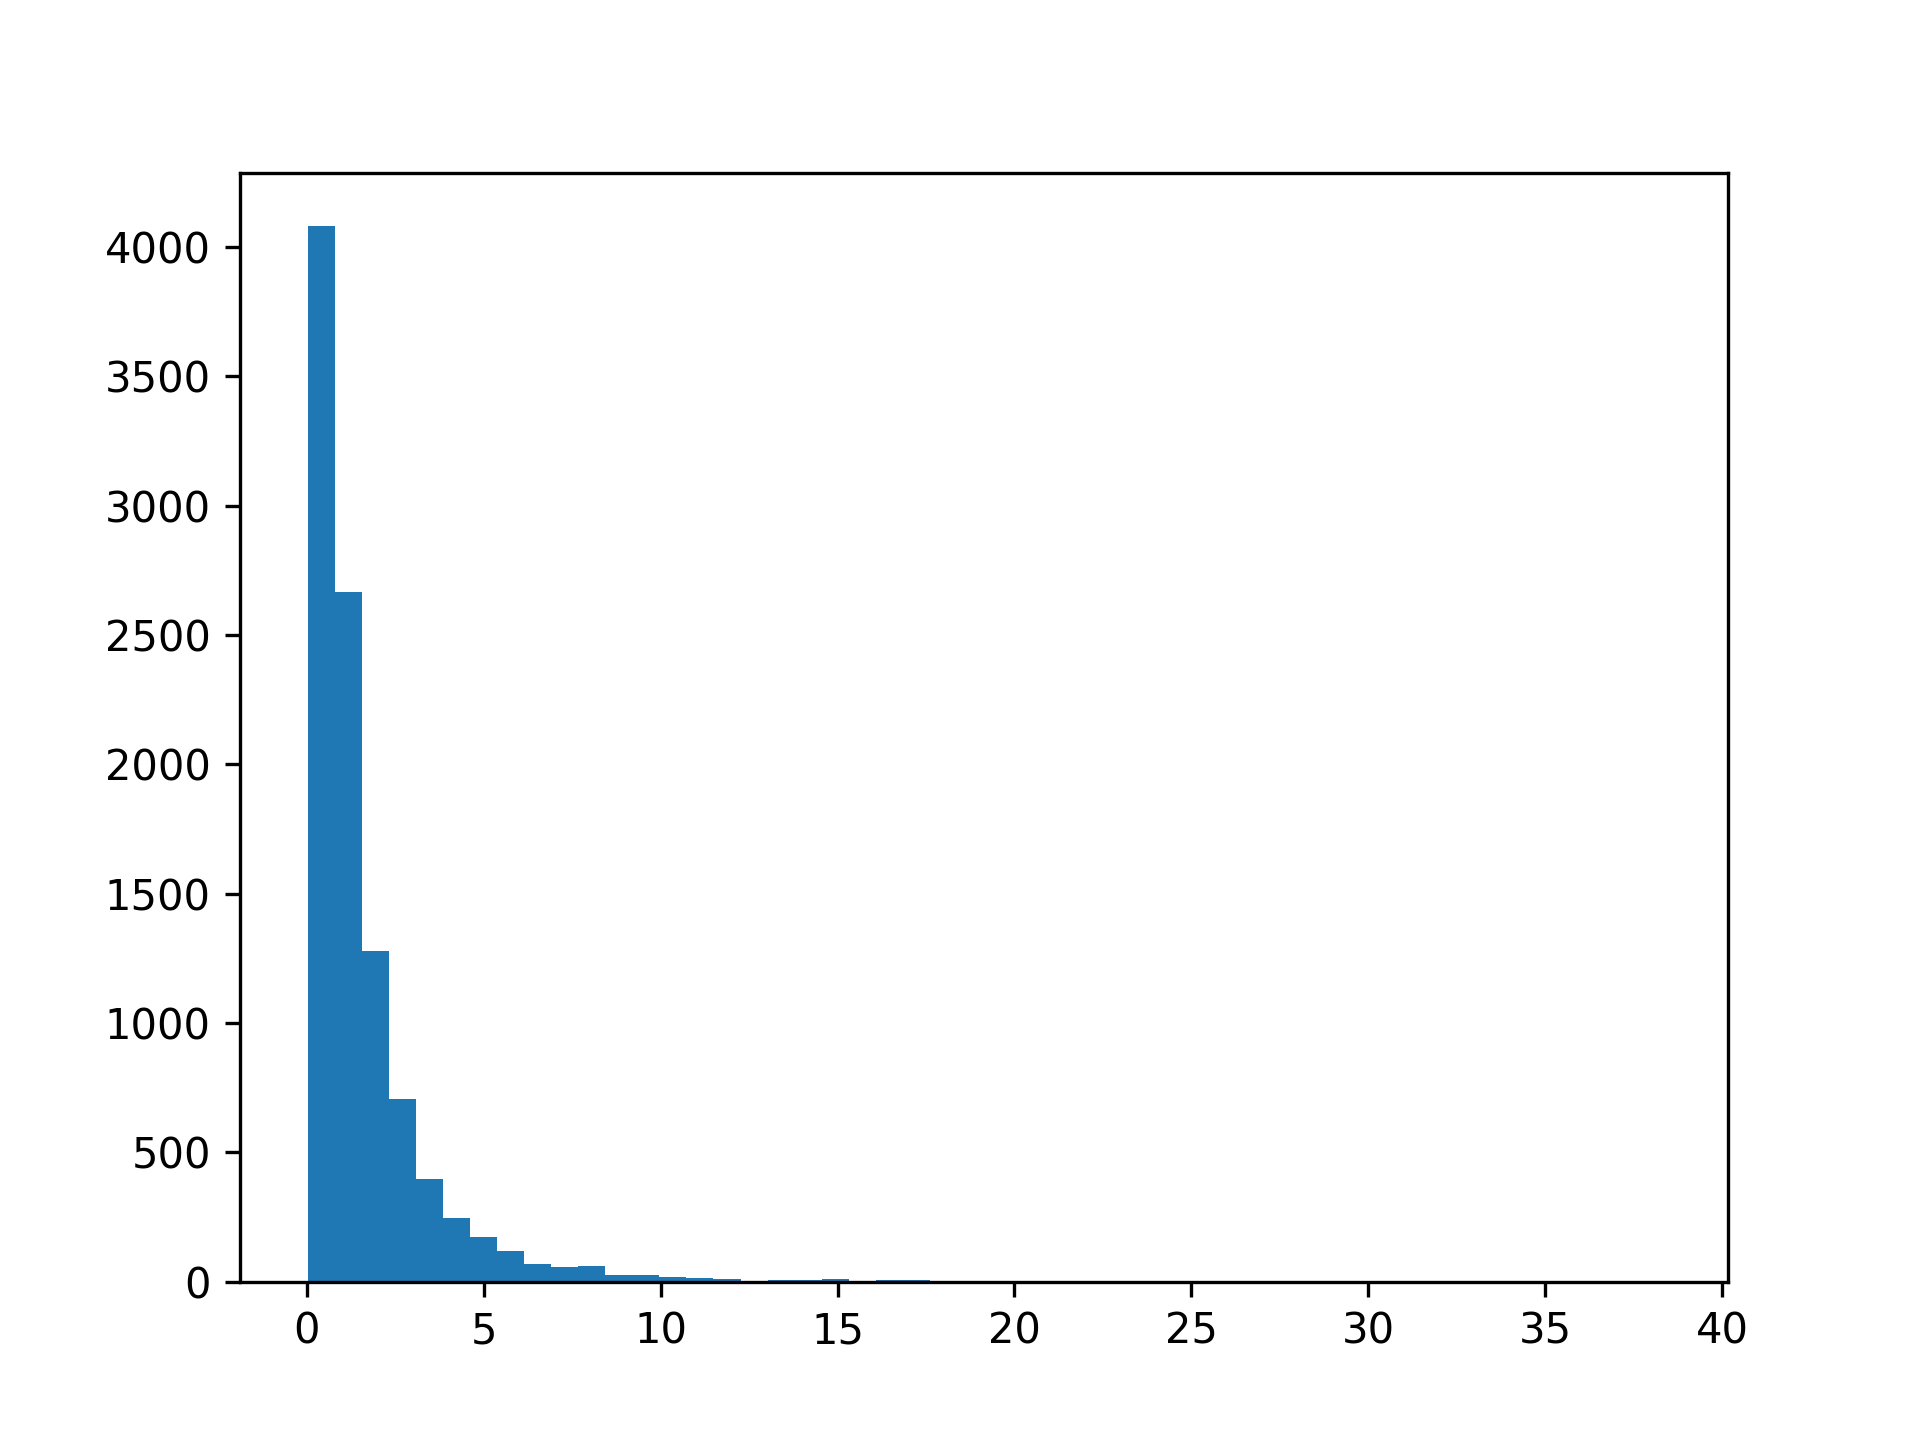
\includegraphics[width=\linewidth]{2-Random_Variables/Ex2_13b.png}
					\end{center}
				\end{itemize}
		\end{enumerate}
	\item Let $(X, Y)$ be uniformly distributed on the unit disk $\{(x, y) : x^2 + y^2 \leq 1\}$. Let $R = \sqrt{X^2 + Y^2}$. Find the CFD and PDF of $R$.
	\item (A univeral random number generator.) Let $X$ have a continuous, strictly increasing CDF $F$. Let $Y = F(X)$. Find the density of $Y$. This is called the probability integral transform. Now, let $U \sim \operatorname{Uniform}(0,1)$ and let $X = F^{-1}(U)$. Show that $X \sim F$. Now write a program that takes Uniform $(0,1)$ random variables and generates random variables from an Exponential $(\lambda)$ distribution.
	\item Let $X \sim \operatorname{Poisson}(\lambda)$ and $Y \sim \operatorname{Poisson}(\mu)$ and assume that $X$ and $Y$ are independent. Show that the dstribution of $X$ given that $X + Y = n$ is $\operatorname{Binomial}(n, \pi)$ where $\pi = \frac{\lambda}{\lambda + \mu}$.
	Hint 1: You may use the following fact: If $X \sim \operatorname{Poisson}(\lambda)$ and $Y \sim \operatorname{Poisson}(\mu)$, and $X$ and $Y$ are independent, then $X + Y \sim \operatorname{Poisson}(\lambda + \mu)$.
	Hint 2: Note that $\{X = x, X + Y = n\} = \{X = x, Y = n - x\}$.
		\begin{itemize}
			\item Recall that
			$$
			P(X = x|X + Y = n) = \frac{P(X = x, X + Y = n)}{P(X + Y = n)}.
			$$
			By the first hint $P(X + Y = n) = \frac{(\lambda + \mu)^n}{n!} e^{-\lambda -\mu}$. Using the second hint we obtain
			$$
			P(X = x, X + Y = n) = P(X = x, Y = n - x),
			$$
			using the independence of $X$ and $Y$ this becomes
			$$
			P(X = x)P(Y = n - x) = \frac{\lambda^x}{x!} e^{-\lambda} \frac{\mu^{n - x}}{(n - x)!}e^{-\mu}.
			$$
			Combining everything then yields
			$$
			\begin{aligned}
			P(X = x|X + Y = n) &= \frac{\frac{\lambda^x}{x!} e^{-\lambda} \frac{\mu^{n - x}}{(n - x)!}e^{-\mu}}{\frac{(\lambda + \mu)^n}{n!} e^{-\lambda-\mu}} \\
			&= \frac{\lambda^x \mu^{n - x}}{(\lambda + \mu)^n} \frac{n!}{x! (n - x)!}
			&= \frac{\lambda^x \mu^{n - x}}{(\lambda + \mu)^n} \binom{n}{x}.
			\end{aligned}
			$$
			Note that if $Z \sim \operatorname{Bin}\left(n, \frac{\lambda}{\lambda + \mu}\right)$ then
			$$
			\begin{aligned}
			P(Z = k) &= \binom{n}{k} \left(\frac{\lambda}{\lambda + \mu}\right)^k \left( 1 - \frac{\lambda}{\lambda + \mu} \right)^{n - k} \\
			&= \binom{n}{k} \left(\frac{\lambda}{\lambda + \mu}\right)^k \left( \frac{\mu}{\lambda + \mu}\right)^{n - k} \\
			&= \frac{n!}{k!(n - k)!} \left(\frac{\lambda}{\lambda + \mu}\right)^k \left( \frac{\mu}{\lambda + \mu}\right)^{n - k}.
			\end{aligned}
			$$
			As such we have shown that $X|X + Y = n \sim \operatorname{Bin}\left(n, \frac{\lambda}{\lambda + \mu}\right)$.
		\end{itemize}
	\item Let
	$$
	f_{X, Y}(x, y) = \begin{cases}
	c(x + y^2),& (x, y) \in [0, 1]^2 \\
	0,& \text{otherwise}.
	\end{cases}
	$$
	Find $P\left(X < \frac{1}{2}| Y = \frac{1}{2}\right)$
	\item let $X \sim \mathcal{N}(3, 16)$. Solve the following using the Normal table and using a computer package.
		\begin{itemize}
			\item Find $P(X < 7)$
			\item Find $P(X > -2)$
			\item Find $x$ such that $P(X > x) = 0.05$.
			\item Find $P(0 \leq X < 4)$.
			\item Find $x$ such that $P(|X| > |x|) = 0.05$.
		\end{itemize}
	\item Prove formula (2.12): When $r$ is strictly monotone increasing or strictly monotone decreasing then $r$ has an inverse $s = r^{-1}$ and in this case one can show that
	$$
	f_Y(y) = f_X(s(y)) \left|\frac{ds(y)}{dy}\right|.
	$$
	\item Let $X, Y \sim \operatorname{Uniform}(0, 1)$ be independent. Find the PDF for $X - Y$ and $X / Y$.
	\item Let $X_1, \dots, X_n \sim \operatorname{Exp}(\beta)$ be iid. Let $Y = \max\{X_1, \dots, X_n\}$. Find the PDF of $Y$. Hint: $Y \leq y$ if and only if $X_i \leq y$ for all $i = 1, \dots, n$.
		\begin{itemize}
			\item To compute the PDF of $Y$, we first determine the CDF of $Y$:
			$$
			\begin{aligned}
			P(Y \leq y) &= P(X_1 \leq y, \dots, X_n \leq y) \\
			&\overset{1}{=} \prod_{i = 1}^n P(X_i \leq y) \\
			&\overset{2}{=} P(X_1 \leq y)^n \\
			&= \left(1 - e^{- \frac{- y}{\beta}}\right),
			\end{aligned}
			$$
			where we have used (1) that the $X_i$ are independent and (2) that they are identically distributed. Differentiating this with respect to $y$ yields
			$$
			\frac{d}{dy} P(Y \leq y) = n (1 - e^{- y / \beta})^{n - 1} \frac{1}{\beta} e^{- y / \beta}.
			$$
		\end{itemize}
\end{enumerate}

\subsection{Expectation}
\begin{enumerate}
	\item Suppose we playa game where we start with $c$ dollars. On each play of the game you either double or halve your money, with equal probability. What is your expected fortune after $n$ trials?
		\begin{itemize}
			\item Let $X_n$ be your money after $n$ trials. Note that
			$$
			E(X_n|X_{n - 1} = k) = \frac{1}{2}(2k + k / 2) = 1.25k,
			$$
			as such
			$$
			E(X_n) = 1.25^n c.
			$$
		\end{itemize}
	\item Show that $Var(X) = 0$ if and only if there is a constant $c$ such that
	$$
	P(X = c) = 1.
	$$
	\item Let $X_1, \dots, X_n \sim \operatorname{Uniform}(0, 1)$ and let $Y_n = \max \{X_1, \dots, X_n\}$. Find $E(Y_n)$.
		\begin{itemize}
			\item We begin by calculating the CDF of $Y$:
			$$
			\begin{aligned}
				F_Y(y) &= P(\max\{X_1, \dots, X_n\} \leq y) \\
				&= P(X_1 \leq s, \dots, X_n \leq x) \\
				&\overset{1}{=} \prod{i = 1}^n P(X_i \leq s) \\
				&\overset{2}{=} P(X_1 \leq s)^n \\
				&= s^n,
			\end{aligned}
			$$
			where we have used (1) that the $X_1, \dots, X_n$ are independent and (2) that they are identically distributed. To obtain the PDF of $Y$ we differentiate this function:
			$$
			f(y) = F_Y'(y) = n s^{n - 1}.
			$$
			Now we can compute the expected value of $Y$ as follows:
			$$
			\int_0^1 x f(x) dx = \int_0^1 x n x^{n - 1} dx = n \int_0^1 x^n dx = \frac{n}{n + 1}. 
			$$
		\end{itemize}
	\item A particle starts at the origin of the real line and moves along the line in jumps of one unit. For each jump the probability is $p$ that the particle will jump one unit to the left and the probability is $1-p$ that the particle
	will jump one unit to the right. Let $X_n$ be the position of the particle after $n$ units. Find $E(X_n)$ and $V(X_n)$. (This is known as a random walk.)
		\begin{itemize}
			\item Note that
			$$
			\begin{aligned}
			E(X_n|X_{n - 1} = k) &= p(k - 1) + (1 - p)(k + 1) \\
			&= (pk - p + k + 1 - pk - p) \\
			&= k + (1 - 2p),
			\end{aligned}
			$$
			as such
			$$
			E(X_n) = n(1 - 2p).
			$$
			[TODO: Do the Variance calculation]
		\end{itemize}
	\item A fair coin is tossed until a head is obtained. What is the expected number of tosses that will be required?
		\begin{itemize}
			\item Note this follows a geometric distribution.
			\item Let $X = k$ denote that the first head appeared on the kth flip. Note that every flip itself is a Bernoulli experiment with $p = 1 - p = 1/2$ as such the probability of heads is always $1/2$. This means that
			$$
			P(X = k) = (1 - 1/2)^{k - 1}(1 / 2) = 2^{-k}.
			$$
			With that we can calculate
			$$
			E(X) = \sum_{k \geq 1} k P(X = k) = \sum_{k \geq 1} k 2^{-k} = 2.
			$$
		\end{itemize}
	\item Prove Theorem 3.6 for discrete random variables
	\item Let $X$ be a continuous random variable with CDF $F$. Suppose that $P(X > 0) = 1$ and that $E(X)$ exists. Show that
	$$
	E(X) = \int_0^\infty P(X > x) dx.
	$$
	Hint: Consider integrating by parts. The following fact is helpful: if $E(X)$ exists then
	$$
	\lim_{x \rightarrow \infty} x [1 - F(x)] = 0.
	$$
	\item Prove Theorem 3.17
	\item (Computer Experiment) Let $X_1, X_2, \dots, X_n$ be $\mathcal{N}(0, 1)$ random variables and let
	$$
	\overline{X}_n = \frac{1}{n} \sum_{i = 1}^n X_i.
	$$
	Plot $\overline{X}_n$ versus $n$ for $n = 1, \dots, 10000$. Repeat for $X_1, X_2, \dots, X_n \sim \operatorname{Cauchy}$. Explain why there is such a difference.
		\begin{itemize}
			\item
			\begin{minted}{python}
import numpy as np
import matplotlib.pyplot as plt

n = 10000

samples = np.random.normal(size = n)
samples_cauchy = np.random.standard_cauchy(size = n)

x = (np.arange(n) + 1)

mean = np.cumsum(samples) / x
mean_cauchy = np.cumsum(samples_cauchy) / x

plt.plot(x, mean, label='Normal Mean')
plt.plot(x, mean_cauchy, label='Cauchy Mean')

plt.legend(loc='upper right')

plt.savefig("Ex3_9.png")
			\end{minted}
			\begin{center}
				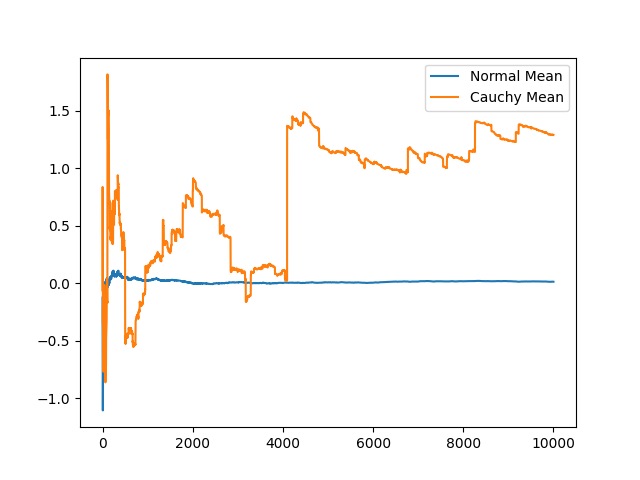
\includegraphics[width=\linewidth]{3-Expectation/Ex3_9.png}
			\end{center}
		\end{itemize}
	\item 
	\item (Computer Experiment: Simulating the Stock Market). Let $Y_1, Y_2, \dots$ be independent random variables such that $P(Y_i = 1) = P(Y_i = -1) = \frac{1}{2}$. Let $X_n = \sum_{i = 1}^n Y_i$. Think of $Y_i = 1$ as "the stock market increased by one dollar", $Y_i = -1$ as "the stock market decreased by one dollar", and $X_n$ as the value of the stock on day $n$.
		\begin{enumerate}
			\item Find $E(X_n)$ and $Var(X_n)$.
				\begin{itemize}
					\item By linearity $E(X_n) = \sum_{i = 1}^n E(Y_i) = \sum_{i = 1}^n (-1)\frac{1}{2} + (1) \frac{1}{2} = 0.$ Note that $E(X_n)^2 = 0$, as such $Var(X_n) = E(X_n^2)$. To calculate this note that
					$$
					X_n^2 = \left( \sum_{i = 1}^n Y_i \right)^2 = \sum_{i = 1}^n Y_i^2 + 2 \sum_{i < j} Y_i Y_j.
					$$
					Because $Y_i \in \{-1, 1\}$ it follows that $E(Y_i^2) = 1$ and as such
					$$
					E(X_n^2) = n + 2 \sum_{i < j} E(Y_i Y_j) = n + 2 \sum_{i < j} P(Y_i Y_j = +1) - P(Y_i Y_j = -1).
					$$
					Note that $Y_i Y_j = 1$ if and only if $(Y_i, Y_j) \in \{(1, 1), (-1, -1)\}$ and $Y_i Y_j = -1$ if and only if $(Y_i, Y_j) \in \{(-1, 1), (1, -1)\}$, as such both of those are equally liked. In total this means that
					$$
					V(X_n) = E(X_n^2) = n.
					$$
				\end{itemize}
			\item Simulate $X_n$ and plot $X_n$ versus $n$ for $n = 1, 2, \dots, 10000$. Repeat the whole simulation several times. Notice two things. First, it's easy to "see" patterns in the sequence even though it is random. Second, you will find that the four runs look very different even though they were generated the same way. How do the calculations in (a) explain the second observation?
				\begin{itemize}
					\item
\begin{minted}{python}
import numpy as np
import matplotlib.pyplot as plt

def Ex3_11(n = 10000, draw = True, save = False, i = 0):
    # 2*0 - 1 = -1, 2 * 1 -1 = 1
    rand = 2 * np.random.randint(low = 0, high = 2, size = n) - 1

    fig, ax = plt.subplots()
    ax.plot(range(0, n), np.cumsum(rand))

    if draw:
        plt.show()

    if save:
        fig.savefig(f"Ex3_11-{i}.png")

for i in range(4):
    Ex3_11(draw = True, save = True, i = i)
\end{minted}
\begin{figure}
  \centering
  \begin{tabular}{cc}
    \begin{subfigure}{0.45\linewidth}
      \centering
      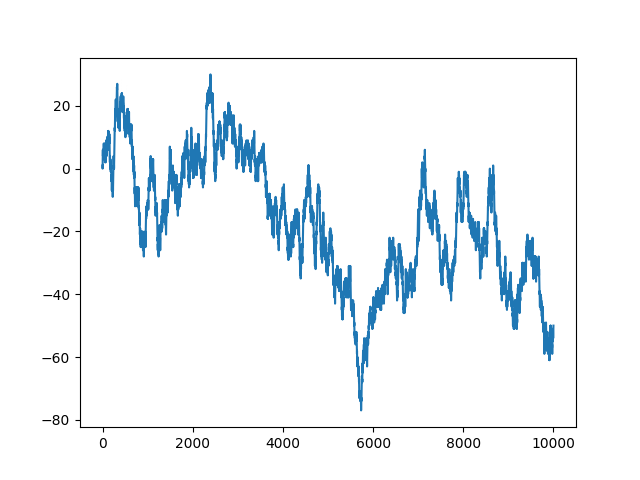
\includegraphics[width=\linewidth]{3-Expectation/Ex3_11-0.png}
      \caption{}
    \end{subfigure}
    &
    \begin{subfigure}{0.45\linewidth}
      \centering
      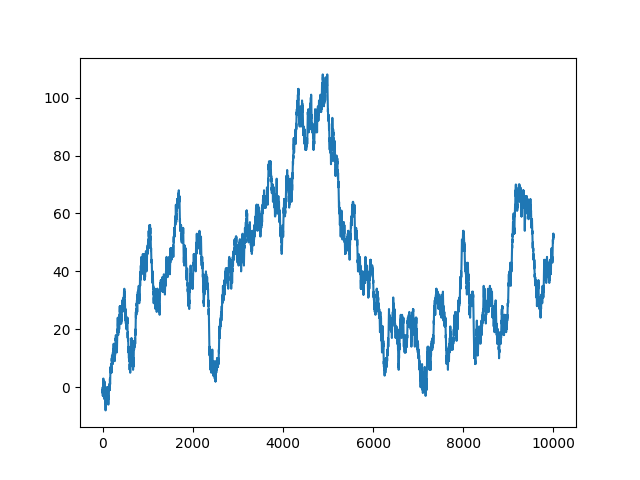
\includegraphics[width=\linewidth]{3-Expectation/Ex3_11-1.png}
      \caption{}
    \end{subfigure}
    \\
    \begin{subfigure}{0.45\linewidth}
      \centering
      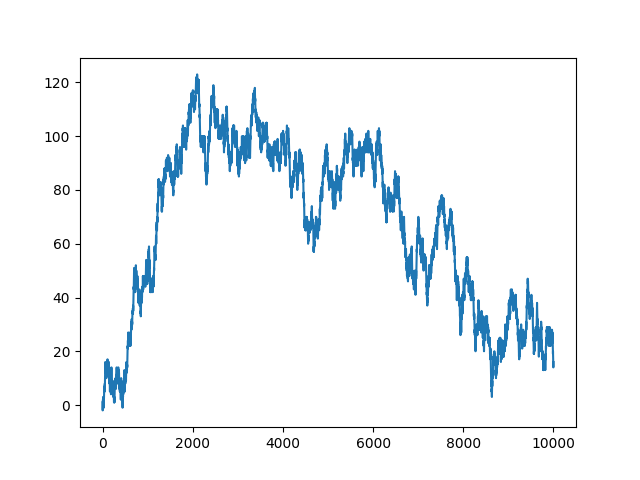
\includegraphics[width=\linewidth]{3-Expectation/Ex3_11-2.png}
      \caption{}
    \end{subfigure}
    &
    \begin{subfigure}{0.45\linewidth}
      \centering
      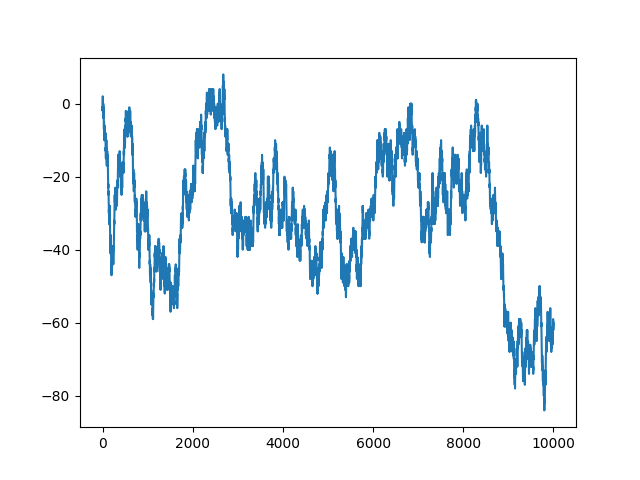
\includegraphics[width=\linewidth]{3-Expectation/Ex3_11-3.png}
      \caption{}
    \end{subfigure}
  \end{tabular}
\end{figure}
				\end{itemize}
		\end{enumerate}
	\item Prove the formulas given in the table at the beginning of Section $3.4$ for the Bernoulli, Poisson, Uniform, Exponential, Gamma, and Beta. Here are some hints. For the mean of the Poisson, use the fact that
	$$
	e^a = \sum_{x = 0}^\infty \frac{a^x}{x!}.
	$$
	To compute the variance, first compute $E(X(X -1))$. For the mean of the Gamma, it will help to multiply and divide by$\Gamma(\alpha + 1)/\beta^{\alpha + 1}$ and use the fact that a Gamma density integrates to $1$. For the Beta, multiply and divide by
	$$
	\frac{\Gamma(\alpha + 1) \Gamma(\beta)}{\Gamma(\alpha + \beta + 1)}.
	$$
	\item 
	\item Let $X_1, \dots, X_m$ and $Y_i, \dots, Y_n$ be random variables and let $a_1, \dots, a_m$ and $b_1, \dots, b_n$ be constants. Show that
	$$
	\operatorname{Cov}\left( \sum_{i = 1}^m a_i X_i, \sum_{j = 1}^n b_j Y_j \right) = \sum_{i = 1}^m \sum_{j = 1}^n a_i b_j \operatorname{Cov}(X_i, Y_j)
	$$
	\item Let
	$$
	f_{X, Y}(x, y) =
	\begin{cases}
	\frac{1}{3}(x + y) & 0 \leq 0 \leq 1, 0 \leq y \leq 2 \\
	0 & \text{otherwise}
	\end{cases}
	$$
	Find $V(2X - 3Y + 8)$.
	\item Let $r(x)$ be a function of $x$ and let $s(y)$ be a function of $y$. Show that
	$$
	E(r(X)s(Y)|X) = r(X)E(s(Y)|X).
	$$
	Also, show that $E(r(X)|X) = r(X)$.
	\item 
	\item Show that if $E(X|Y = y) = c$ for some constant $c$, then $X$ and $Y$ are uncorrelated.
	\item 
	\item Prove Lemma 3.21.
	\item Let $X$ and $Y$ be random variables. Suppose that $E(Y|X) = X$. Show that $\operatorname{Cov}(X, Y) = V(x)$.
	\item
	\item Find the moment generating function for the Poisson, Normal, and Gamma distributions.
	\item Let $X_1, \dots, X_n \sim \operatorname{Exp}(\beta)$. Find the moment generating function of $X_i$. Prove that
	$$
	\sum_{i = 1}^n X_i \sim \operatorname{Gamma}(n, \beta).
	$$
\end{enumerate}

\subsection{Inequalities}
\begin{enumerate}
	\item Let $X \sim \operatorname{Exp}(\beta)$. Find $P(|X - \mu_X| \geq k \sigma_X)$ for $k > 1$. Compare this to the bound you get from Chebyshev's inequality.
	\item Let $X \sim \operatorname{Po}(\lambda)$. Use Chebyshev's inequality to show that $P(X \geq 2\lambda) \leq \frac{1}{\lambda}$.
	\item Let $X_1, \dots, X_n \sim \operatorname{Bernoulli}(p)$ (note this is just $\operatorname{Bin}(1, p)$) and
	$$
	\overline{X}_n = \frac{1}{n} \sum_{i = 1}^n X_i.
	$$
	Bound $P(|\overline{X}_n - p| > \varepsilon)$ using Chebychev's inequality and using Hoeffding's inequality. Show that, when $n$ is large, the bound from Hoeffding's inequality is smaller than the bound from Chebychev's inequality.
	\item Let $X_1, \dots, X_n \sim \operatorname{Bernoulli}(p)$.
		\begin{enumerate}
			\item Let $\alpha > 0$ be fixed and define
			$$
			\varepsilon_n = \sqrt{\frac{1}{2n}\log\left(\frac{2}{\alpha}\right)}.
			$$
			Let $\overline{X}_n = \frac{1}{n}\sum_{i = 1}^n X_i$. Define $C_n = (\overline{X}_n - \varepsilon, \overline{X}_n + \varepsilon)$. Use Hoeffding's inequality to show that
			$$
			P(C_n\text{ contains }p) \geq 1 - \alpha.
			$$
			In practice, we truncate the interval so it does not go below $0$ or above 1.
				\begin{itemize}
					\item Let
					$$
					\varepsilon_n = \sqrt{\frac{1}{2n} \log\left(\frac{2}{\alpha}\right)},
					$$
					then
					$$
					\varepsilon_n^2 = \frac{1}{2n} \log\left(\frac{2}{\alpha}\right).
					$$
					With that we can then calculate
					$$
					\begin{aligned}
					e^{-2n\varepsilon^2} &= e^{- 2n \frac{1}{2n} \log\left( \frac{2}{\alpha} \right)} \\
					&= e^{- \log \left( \frac{2}{\alpha} \right)} \\
					&= e^{\log\left( \frac{\alpha}{2} \right)} \\
					&= \frac{\alpha}{2}.
					\end{aligned}
					$$
					Recall that Hoeffding's inequality (the bernoulli case) states that
					$$
					P(|\overline{X}_n - p| > \varepsilon_n) \leq 2e^{-2n \varepsilon_n^2}.
					$$
					As such
					$$
					P(|\overline{X} - p| > \varepsilon_n) \leq \alpha.
					$$
					The left hand side is
					$$
					\begin{aligned}
					1 - P(|\overline{X}_n - p| &\leq \varepsilon_n) \\
					&= 1 - P(\overline{X}_n - \varepsilon \leq p \leq \overline{X}_n + \varepsilon) \\
					&= 1 - P(p \in C_n) = 1 - P(C_n\text{ contains }p).
					\end{aligned}
					$$
					Putting everything together yields
					$$
					1 - \alpha \leq P(C_n\text{ contains }p).
					$$
				\end{itemize}
			\item (Computer Experiment) Let's examine the properties of this confidence interval. Let $\alpha = 0.05$ and $p = 0.4$. Conduct a simulation study to see how often the interval contains $p$ (called the coverage). Do this for various values of $n$ between $1$ and $10000$. Plot the coverage versus $n$.
			\begin{itemize}
				\item For code see the next subproblem.
				\begin{center}
					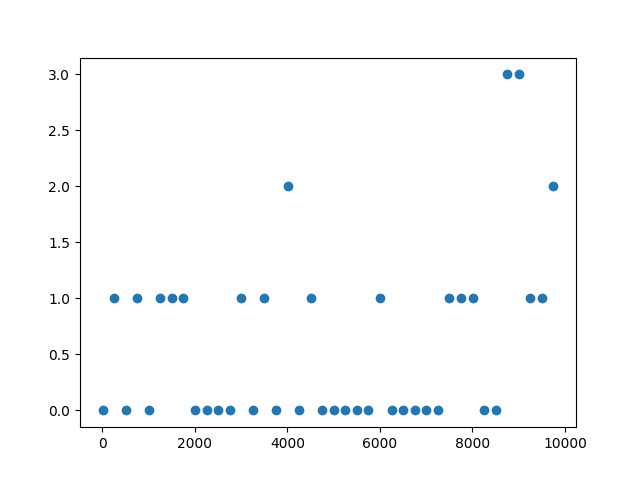
\includegraphics[width=\linewidth]{4-Probability_Inequalities/Ex4_4b.png}
				\end{center}
			\end{itemize}
			\item Plot the length of the interval versus $n$. Suppose we want the length of the interval to be no more than $0.05$. How large should $n$ be?
				\begin{itemize}
					\item 
					\begin{minted}{python}
import numpy as np
import matplotlib.pyplot as plt

n_list = np.arange(start=1, step=250, stop=10000, dtype=int)
alpha = 0.05
p = 0.4

coverages, lengths = {}, {}
for n in n_list:
    eps = np.sqrt(np.log(2 / alpha) / (2 * n))

    coverage, length = 0, []
    for i in range(100):
        X = np.random.binomial(n = 1, p = p, size = n)
        mean = np.mean(X)
        
        if (p < (mean - eps)) or (p > (mean + eps)):
            coverage += 1

        length.append(2 * eps) 

    coverages[n] = coverage
    lengths[n] = np.mean(length)

x = list(coverages.keys())
y_cov = list(coverages.values())
y_len = list(lengths.values())

plt.scatter(x, y)
plt.savefig("Ex4_4b.png")
plt.cla()
plt.plot(x[1:], y_len[1:]) # First length skews the plot heavily
plt.plot(x[1:], [0.05]*(len(x[1:]))) # Horizontal Line
plt.savefig("Ex4_4c.png")
					\end{minted}
					\begin{center}
						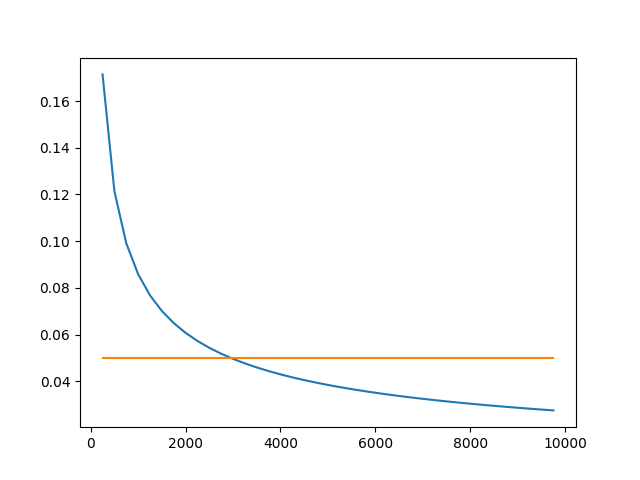
\includegraphics[width=\linewidth]{4-Probability_Inequalities/Ex4_4c.png}
					\end{center}
				\end{itemize}
		\end{enumerate}
	\item Prove Mill's Inequality, Theorem 4.7. Hint. Note that $P(|Z| > t) = 2P(Z > t)$. Now write out what $P(Z > t)$ means and note that $x / t > 1$ whenever $x > t$.
	\item Let $Z \sim N(0, 1)$. Find $P(|Z| > t)$ and plot this as a function of $t$. From Markov's inequality, we have the bound
	$$
	P(|Z| > t) \leq \frac{E(|Z|^k)}{t^k}
	$$
	for any $k > 0$. Plot these bounds for $k = 1, \dots, 5$ and compare them to the true value of $P(|Z| > t)$. Also, plot the bound from Mill's inequality.
	\item Let $X_1, \dots, X_n \sim N(0, 1)$. Bound $P(|\overline{X}_n| > t)$ using Mill's inequality, where
	$$
	\overline{X}_n = \frac{1}{n} \sum_{i = 1}^n X_i.
	$$
	Compare to the Chebyshev bound.
\end{enumerate}

\subsection{Convergence of Random Variable}
\begin{enumerate}
	\item
	\item Let $X_1, X_2, \dots$ be a sequence of random variables.Show that $X_n \overset{qm}{\longrightarrow} b$ if and only if
	$$
	\begin{aligned}
	\lim_{n \rightarrow \infty} E(X_n) = b,&&\lim_{n \rightarrow \infty}V(X_n) = 0.
	\end{aligned}
	$$
	\item Let $X_1, \dots, X_n$ be IID and let $\mu := E(X_1)$. Suppose that the variance is finite. Show that $\overline{X}_n \overset{qm}{\longrightarrow} \mu$
	\item Let $X_1, X_2, \dots$ be a sequence of random variables such that
	$$
	\begin{aligned}
	P\left(X_n = \frac{1}{n}\right) = 1 - \frac{1}{n^2},&& P(X_n = n) \frac{1}{n^2}
	\end{aligned}
	$$
	Does $X_n$ converge in probability? Does $X_n$ converge in quadratic mean?
	\item Let $X_1, \dots, X_n \sim \operatorname{Bernoulli}(p)$. Prove that
	$$
	\begin{aligned}
	\frac{1}{n} \sum_{i = 1}^n X_i^2 \overset{P}{\longrightarrow} p,&& \frac{1}{n}\sum_{i = 1}^n X_i^2 \overset{qm}{\longrightarrow} p.
	\end{aligned}
	$$
	\item Suppose that the height of men has mean $68$ inches and standard deviation $2.6$ inches. We draw $100$ men at random. Find (approximately) the probability that the average height of men in our sample will be at least $68$ inches.
	\item Let $\lambda_n = 1 / n$ for $n = 1, 2, \dots$. Let $X_n \sim \operatorname{Poisson}(\lambda_n)$.
		\begin{enumerate}
			\item Show that $X_n \overset{P}{\longrightarrow} 0$.
			\item Let $Y_n = nX_n$. Show that $Y_n \overset{P}{\longrightarrow} 0$.
		\end{enumerate}
	\item Suppose we have a computer program consisting of $n = 100$ pages of code. Let $X_i$ be the number of errors on the $i$th page of code. Suppose that the $X_i$ are Poisson with mean $1$ and that they are independent. Let
	$$
	Y = \sum_{i = 1}^n X_i
	$$
	be the total number of errors. Use the central limit theorem to approximate
	$$
	P(Y < 90).
	$$
	\item
	\item Let $Z \sim N(0, 1)$. Let $t > 0$. Show that, for any $k > 0$,
	$$
	P(|Z| > t) \leq \frac{E|Z|^k}{t^k}.
	$$
	Compare this to Mill's inequality in Chapter 4.
	\item Suppose that $X_n \sim N(0, 1/n)$ and let $X$ be a random variable with distribution $F(x) = 0$ if $x < 0$ and $F(x) = 1$ if $x \geq 1$. Does $X_n$ converge to $X$ in probability? (Prove or disprove). Does $X_n$ converge to $X$ in distribution? (Prove or disprove).
	\item Let $X, X_1, X_2, X_3, \dots$ be random variables that are positive and integer valued. Show that $X_n \leadsto X$ if and only if
	$$
	\lim_{n \rightarrow \infty} P(X_n = k) = P(X = k)
	$$
	for every integer $k$.
	\item
	\item Let $X_1, \dots, X_n \sim \operatorname{Uniform}(0, 1)$. Let $Y_n = \overline{X}_n^2$. Find the limiting distribution of $Y_n$.
	\item
	\item Construct an example where $X_n \leadsto X$ and $Y_n \leadsto Y$ but $X_n + Y_n$ does not converge in distribution to $X + Y$.
\end{enumerate}

\section{Statistical Inference}
\subsection{Models, Statistical Inference and Learning}
\begin{enumerate}
	\item Let $X_1, \dots, X_n \sim \operatorname{Poisson}(\lambda)$ and let $\hat{\lambda} = \frac{1}{n} \sum_{i = 1}^n$. Find the $\bias$, $\se$, and $\mse$ of this estimator.
		\begin{itemize}
			\item Recall that $E_\lambda$ is linear and that the expected value of $X \sim \operatorname{Po}(\lambda)$ is $\lambda$. As such
			$$
			E_\lambda(\hat{\lambda}_n) = \frac{1}{n} \sum_{i = 1}^n E(X_i) = \frac{1}{n} n \lambda = \lambda.
			$$
			This means that $\bias = 0$, i.e., this estimator is unbiased.
			\item Similiarly, the variance of $X \sim \operatorname{Po}(\lambda)$ is equal to $\lambda$, as such $se^2 = \lambda / n$. To see this note that $Var(aX) = a^2Var(X)$, i.e.,
			$$
			se = \sqrt{\lambda / n}.
			$$
			\item By Theorem 6.9 the mean square error is equal to
			$$
			\mse = \bias^2(\hat{\lambda}_n) + se^2(\hat{\lambda}_n) = \frac{\lambda}{n}.
			$$
		\end{itemize}
	\item Let $X_1, \dots, X_n \sim \operatorname{Uniform}(0, \theta)$ and let $\hat{\theta} = \max\{X_1, \dots, X_n\}$. Find the $\bias$, $\se$, and $\mse$ of this estimator.
		\begin{itemize}
			\item We begin by determining the CDF of $\hat{\theta}$.
			$$
			\begin{aligned}
			F_{\hat{\theta}}(x) &= F(\hat{\theta} \leq x) \\ 
			&= F(\max\{X_1, \dots, X_n\} \leq x) \\
			&= F(X_1 \leq x, X_2 \leq x, \dots, X_n \leq x) \\
			&\overset{1}{=} \prod_{i = 1}^n F(X_i \leq x) \\
			&\overset{2}{=} (F(X_i \leq x))^n \\
			&= \left( \frac{x}{\theta} \right)^n \\
			&= \frac{x^n}{\theta^n},
			\end{aligned}
			$$
			where we have used (1) the independence of the random variables and (2) the fact that they are identically distributed. To obtain the PDF we differentiate with respect to $x$ to obtain
			$$
			\begin{aligned}
			f_{\hat{\theta}}(x) &= \frac{\partial}{\partial x} F_{\hat{\theta}}(x) \\
			&= \frac{\partial}{\partial x} \frac{x^n}{\theta^n} \\
			&= n \frac{x^{n - 1}}{\theta^n}.
			\end{aligned}
			$$
			With that we can now calculate the expected value
			$$
			\begin{aligned}
			E_\theta(\hat{\theta}) &= \int_0^\theta x (n x^{n-1} / \theta^n) dx \\
			&= n \int_0^\theta \frac{x^{n}}{\theta^n} dx \\
			&= \frac{n}{\theta^n} \int_0^\theta x^n dx \\
			&= \frac{n}{\theta^n} \left[ \frac{x^{n+1}}{n+1} \right]_0^\theta \\
			&= \frac{n}{n+1} \theta,
			\end{aligned}
			$$
			and
			$$
			\begin{aligned}
			\bias &= E_\theta(\hat{\theta}) - \theta \\
			&= \frac{n}{n+1} \theta - \theta \\
			&= \theta\left(\frac{n}{n+1} - 1\right) \\
			&= -\frac{\theta}{n+1}.
			\end{aligned}
			$$
			\item To compute the standard error we first calculate the second moment of $\hat{\theta}$:
			$$
			\begin{aligned}
			E_\theta(\hat{\theta}^2) &= \int_0^\theta x^2 \frac{n x^{n - 1}}{\theta^n} dx \\
			&= \frac{n}{\theta^n} \int_0^\theta x^{n + 1} dx \\
			&= \frac{n}{\theta^n} \left. \frac{1}{n + 2} x^{n + 2} \right|_{x = 0}^{x = \theta} \\
			&= \frac{n}{\theta^n} \frac{\theta^{n + 2}}{n + 2} \\
			&= \frac{n}{n + 2} \theta^2.
			\end{aligned}
			$$
			As such
			$$
			V(\hat{\theta}) = E_\theta(\hat{\theta}^2) - E_\theta(\hat{\theta})^2 = \frac{n}{n + 2} \theta^2 - \frac{\theta^2}{(n+1)^2}
			$$
			and
			$$
			\se(\hat{\theta}) = \sqrt{V(\hat{\theta})} = \sqrt{\frac{n}{n + 2} - \frac{1}{(n + 1)^2}}\theta.
			$$
			\item By Theorem 6.9 it follows
			$$
			\begin{aligned}
			\mse(\hat{\theta}) &= \bias^2(\hat{\theta}) + V(\hat{\theta}) \\
			&= \frac{\theta^2}{(n + 1)^2} + \frac{n}{n + 2}\theta^2 - \frac{\theta^2}{(n + 1)^2} \\
			&= \frac{n}{n + 2}\theta^2.
			\end{aligned}
			$$
		\end{itemize}
	\item Let $X_1, \dots, X_n \sim \operatorname{Uniform}(0, \theta)$ and let $\hat{\theta} = 2 \overline{X}_n$. Find the $\bias$, $\se$, and $\mse$ of this estimator.
\end{enumerate}

\subsection{Estimating the CDF and Statistical Functionals}
\begin{enumerate}
	\item Prove Theorem 7.3.
		\begin{itemize}
			\item First of all note that
			$$
			E(I(X_i \leq x)) = 1 \cdot P(X_i \leq x) + 0 \cdot P(X_i > 0) = F(x)
			$$
			holds, with that we can calculate
			$$
			\begin{aligned}
			E(\hat{F}_n(x)) &= \frac{1}{n} \sum_{i = 1}^n E(I(X_i \leq x)) \\
			&= \frac{1}{n} \sum_{i = 1}^n F(x) = F(x).
			\end{aligned}
			$$
			\item To compute the variance we first want to calculate the second moment of $\hat{F}_n(X)$. First of all note that $I(X_i \leq x)^2 = I(X_i \leq x) = F(x)$. Using this we now calculate the second moment:
			$$
			\begin{aligned}
			E(\hat{F}_n^2(X)) &= E\left( \frac{1}{n^2} \left( \sum_{i = 1}^n I(x_i \leq x) \right)\right) \\
			&= E\left( \frac{1}{n^2} \sum_{i = 1}^n I(x_i \leq x)^2 + \frac{1}{n^2} \sum_{i < j} I(X_i \leq x)I(X_j \leq x) \right) \\
			&= \frac{1}{n} E\left( \frac{1}{n} \sum_{i = 1}^n I(X_i \leq x)) \right) + \frac{1}{n^2} \sum_{i < j} E(I(X_i \leq x)I(X_j \leq x)) \\
			&= \frac{F(x)}{n} + \frac{1}{n^2} \sum_{i < j} P(I(X_i \leq x)I(X_j \leq x) = 1) \\
			&= \frac{F(x)}{n} + \frac{1}{n^2} \sum_{i < j} P(I(X_i \leq x) = 1, P(I(X_j \leq x) = 1) \\
			&= \frac{F(x)}{n} + \frac{1}{n^2} \sum_{i < j} P(X_i \leq x)P(X_j \leq x) \\
			&= \frac{F(x)}{n} + \frac{1}{n^2} \sum_{i < j} F(x)^2 \\
			&= \frac{F(x)}{n} + \frac{1}{n^2} \frac{n(n - 1)}{2} F(x)^2 \\
			&= \frac{F(x)}{n}\left(1 + \frac{n - 1}{2} F(x)^2 \right).
			\end{aligned}
			$$
			We have already computed the expected value of $\hat{F}_n$. In total the variance then is
			$$
			\begin{aligned}
			V(\hat{F}_n(x)) &= E(\hat{F}_n^2(x)) - E(\hat{F}_n(x))^2 \\
			&= \frac{F(x)}{n}\left(1 + \frac{n - 1}{2} F(x)^2 \right) - F(x)^2 \\
			&= \frac{F(x)(1 - F(x))}{n}.
			\end{aligned}
			$$
			\item Note that the bias is equal to $0$, as such by Theorem 6.9
			$$
			\mse(\hat{F}_n(x)) = V(\hat{F}_n(x)).
			$$
			\item We want to show that for all $\varepsilon > 0$
			$$
			P(|\hat{F}_n(x) - F(x)| > \varepsilon) \rightarrow 0
			$$
			as $n \rightarrow \infty$. Note that $F(x) = E(\hat{F}_n(x))$. Applying Theorem 4.2 (Chebyshev's Inequality) we get
			$$
			P(|\hat{F}_n(x) - F(x)| > \varepsilon) \leq \frac{V(\hat{F}_n(x)}{\varepsilon^2}
			$$
			and by including the variance
			$$
			P(|\hat{F}_n(x) - F(x)| > \varepsilon) \leq \frac{\frac{F(x)(1 - F(x))}{n}}{\varepsilon^2},
			$$
			which is equivalent to
			$$
			P(|\hat{F}_n(x) - F(x)| > \varepsilon) \leq \frac{1}{n} \frac{F(x)(1 - F(x))}{\varepsilon^2} \rightarrow 0
			$$
			as $n \rightarrow \infty$. As such $\hat{F}_n(x) \overset{P}{\rightarrow} F(x)$.
		\end{itemize}
	\item Let $X_1, \dots, X_n \sim \Bernoulli(p)$ and let $Y_1 , ... , Y_m \sim \Bernoulli(q)$. Find the plug-in estimator and estimated standard error for $p$. Find an approximate $90$ percent confidence interval for $p$. Find the plug-in estimator and estimated standard error for $p - q$. Find an approximate $90$ percent confidence interval for $p - q$.
		\begin{itemize}
			\item Note that $Y_n := \sum_{i = 1}^n X_i \sim \Bin(n, p)$ and therefore $E(Y_n) = np$ and $V(Y_n) = np(1 - p)$. Furthermore note that the mean
			$$
			\overline{X}_n := \frac{1}{n} Y_n
			$$
			satisfies $E(\overline{X}_n) = \frac{1}{n}E(Y_n) = p$ by linearity. This is our plug-in estimator. The variance is
			$$
			V(\overline{X}_n) = \frac{p(1 - p)}{n},
			$$
			as such the standard error of this estimator is
			$$
			\se(\overline{X}_n) = \sqrt{\frac{p(1 - p)}{n}}.
			$$
			\item This allows us to define the (Normal-based) confidence interval by using (7.6):
			$$
			(p - z_{\alpha / 2} \se, p + z_{\alpha / 2} \se)
			$$
			and observing that for a $95\%$ confidence interval $z_{\alpha / 2} = z_{0.05/2} = 1.96 \approx 2$ we get
			$$
			\left(p - 2\sqrt{\frac{p(1 - p)}{n}}, p + 2\sqrt{\frac{p(1 - p)}{n}}\right).
			$$
			\item
\begin{minted}{python}
import numpy as np
import matplotlib.pyplot as plt
from Scripts.plots import *

def generateConfidence(n, p):
    se = np.sqrt((p * (1 - p)) / n)
    conf = [p - 2 * se, p + 2 * se]
    inConf = lambda x : (x > conf[0]) & (x < conf[1])
    return conf, inConf

def countSamples(q_list, n = 50, p = 0.3, num_samples = 100000):
    y = []
    for q in q_list:
        mu = np.random.binomial(n=n, p=q, size=num_samples) / n
        count = np.sum(inConf(mu))
        y.append(count / num_samples)
    return y

num_samples = 100000
step_size = 0.02
p_list = [0.1, 0.3, 0.5, 0.7, 0.95]
for p in p_list:
    n = 50
    conf, inConf = generateConfidence(n = n, p = p)

    q_list = np.arange(start=0, stop=1, step=step_size)
    y = countSamples(n = n, p = 0, num_samples = num_samples, q_list = q_list)
    plt.plot(q_list, y, label=f'p = {p}')

plot7_2_1(save = True)

n_list = [10, 25, 50, 100]
p = 0.3
for n in n_list:
    conf, inConf = generateConfidence(n = n, p = p)

    q_list = np.arange(start=0, stop=1, step=step_size)
    y = countSamples(n = n, p = 0, num_samples = num_samples, q_list = q_list)

    plt.plot(q_list, y, label=f'p = {p}')

    plot7_2_2(save = True, n = n, p = p, conf = conf)
\end{minted}
		\item
\begin{center}
\begin{tabular}{cc}
    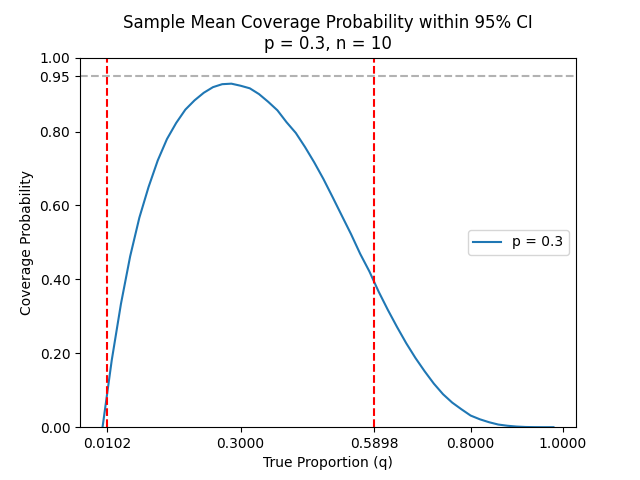
\includegraphics[width=0.5\textwidth]{7-Estimating_the_CDF_and_Statistical_Functionals/Ex7_2_2-10.png} &
    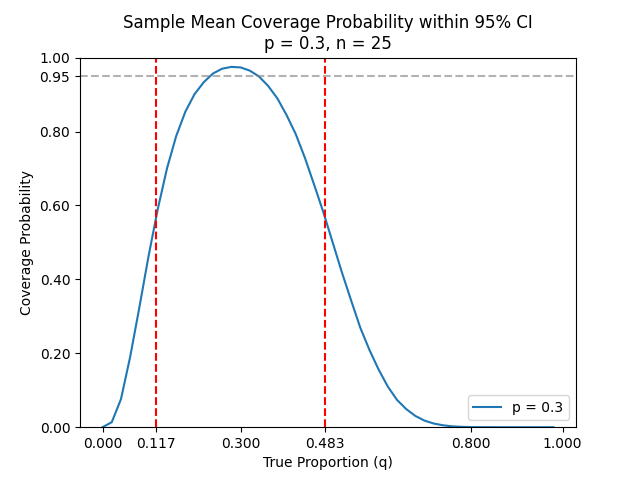
\includegraphics[width=0.5\textwidth]{7-Estimating_the_CDF_and_Statistical_Functionals/Ex7_2_2-25.png} \\
    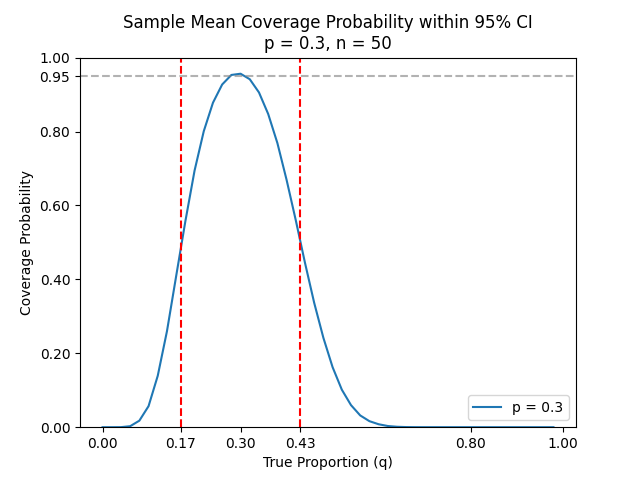
\includegraphics[width=0.5\textwidth]{7-Estimating_the_CDF_and_Statistical_Functionals/Ex7_2_2-50.png} &
    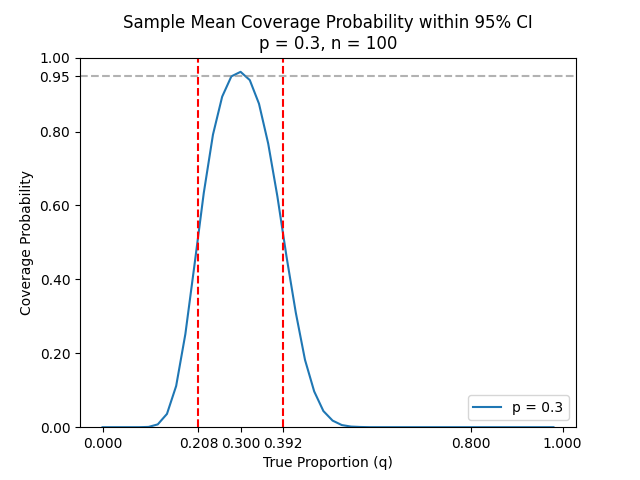
\includegraphics[width=0.5\textwidth]{7-Estimating_the_CDF_and_Statistical_Functionals/Ex7_2_2-100.png}
\end{tabular}
\end{center}

\begin{center}
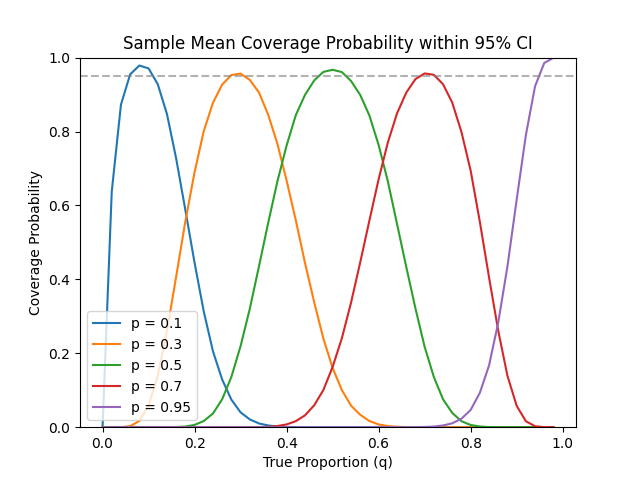
\includegraphics[width=0.6\textwidth]{7-Estimating_the_CDF_and_Statistical_Functionals/Ex7_2_1.png}
\end{center}
		\end{itemize}
	\item (Computer Experiment) Generate $100$ observations from a $\mathcal{N}(0, 1)$ distribution. Compute a $95$ percent confidence band for the CDF $F$ (as described in the appendix). Repeat this $1000$ times and see how often the confidence band contains the true distribution function. Repeat using data from a Cauchy distribution.
		\begin{itemize}
			\item
			\begin{minted}{python}
import numpy as np
import scipy
import matplotlib.pyplot as plt
# Allows to use Latex Code
plt.rcParams.update({
    "text.usetex": True
})

rng = np.random.default_rng()

n, alpha = 100, 0.05
samples = rng.normal(size = n)
eps = np.sqrt(np.log(2 / alpha)  / (2 * n))

F = lambda x : (sum(samples < x) / 100)
L = lambda x : np.maximum(F(x) - eps, 0)
U = lambda x : np.minimum(F(x) + eps, 1)
N = scipy.stats.norm.cdf

X = np.arange(start = -4, stop = 4, step = 0.1)
yF = np.vectorize(F)(X)
yL = np.vectorize(L)(X)
yU = np.vectorize(U)(X)
yN = np.vectorize(N)(X)

plt.plot(X, yL, label = "L(x)")
plt.plot(X, yF, label = r"$\hat{F}_n(x)$")
plt.plot(X, yU, label = "U(x)")
plt.plot(X, yN, linestyle='--', label = r"$\Phi(x)$")

plt.legend()
plt.legend(fontsize=14)

plt.savefig("Ex7_3.png", dpi = 300)
plt.show()
			\end{minted}
			\begin{center}
				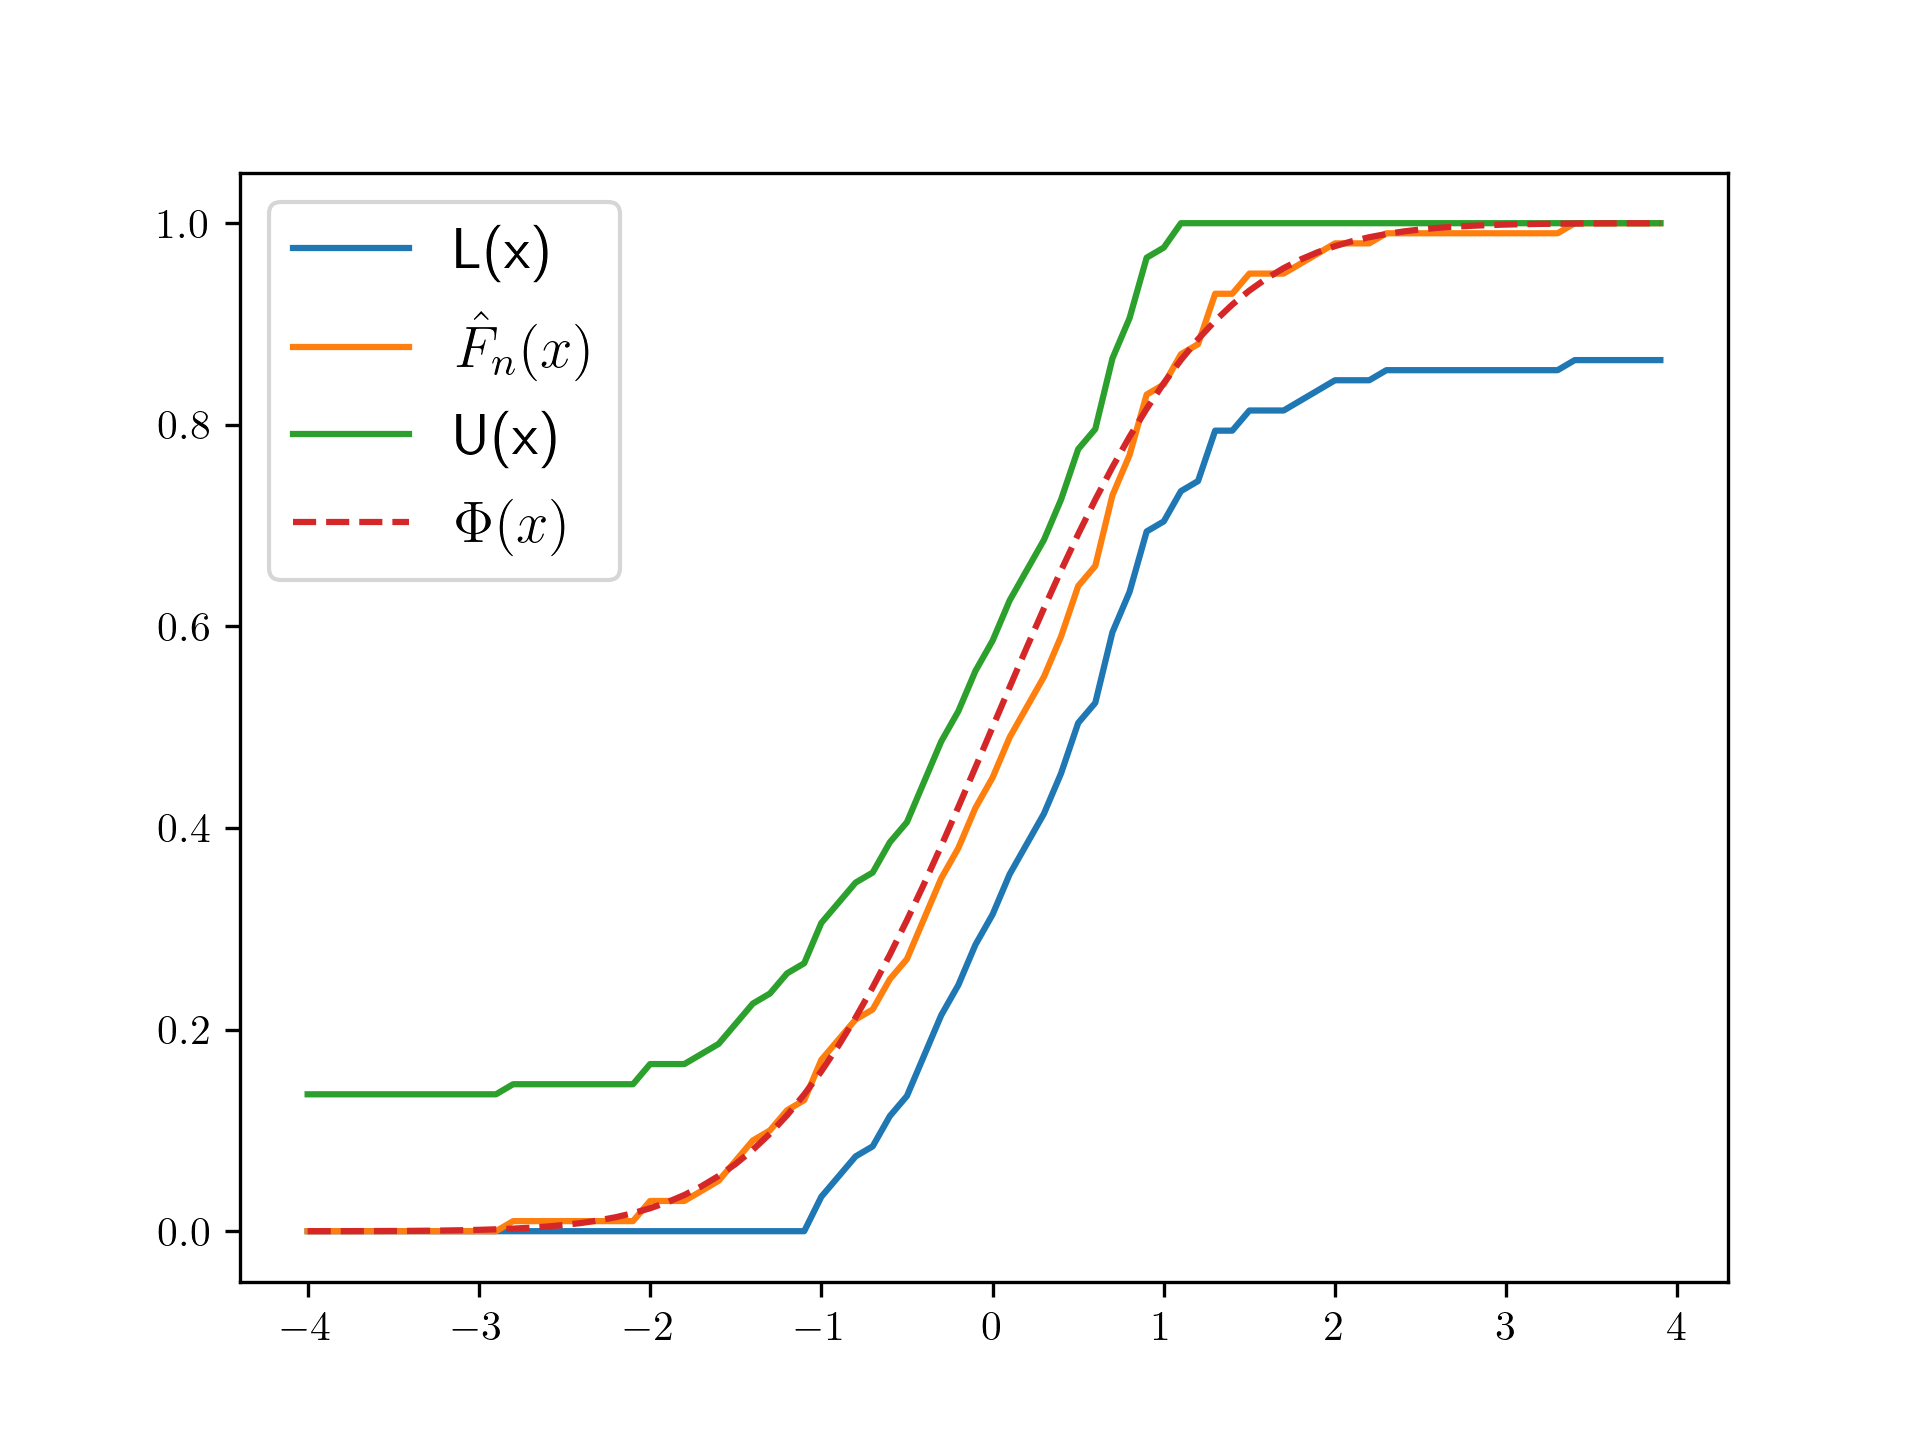
\includegraphics[width=\linewidth]{7-Estimating_the_CDF_and_Statistical_Functionals/Ex7_3.png}
			\end{center}
			\begin{minted}{python}
k, count, count_cauchy = 1000, 0, 0
for i in range(k):
    samples = rng.normal(size = n)
    samples_cauchy = rng.standard_cauchy(size = n)

    F = lambda x : (sum(samples < x) / 100)
    F_cauchy = lambda x : (sum(samples_cauchy < x) / 100)
    L = lambda x : np.maximum(F(x) - eps, 0)
    U = lambda x : np.minimum(F(x) + eps, 1)

    C = scipy.stats.cauchy.cdf

    yF = np.vectorize(F)(X)
    yC = np.vectorize(C)(X)
    yL = np.vectorize(L)(X)
    yU = np.vectorize(U)(X)

    cmp = lambda x : (N(x) >= L(x) and N(x) <= U(x))
    cmp_cauchy = lambda x : (C(x) >= L(x) and C(x) <= U(x))
    contains = np.vectorize(cmp)(X)
    contains_cauchy = np.vectorize(cmp_cauchy)(X)
    if not contains.all():
        count += 1

    if not contains_cauchy.all():
        count_cauchy += 1

print(f"Normal : {count / k * 100:.2f}%")
print(f"Cauchy : {count_cauchy / k * 100:.2f}%")

> Normal : 2.30%
> Cauchy : 84.60%
			\end{minted}
		\end{itemize}
	\item Let $X_1, \dots, X_n \sim F$ and let $\hat{F}(x)$ be the empirical distribution function. For a fixed $x$, use the central limit theorem to find the limiting distribution of $\hat{F}_n(x)$.
	\item Let $x$ and $y$ be two distinct points. Find $\operatorname{Cov}(\hat{F}_n(x), \hat{F}_n((y)))$.
	\item Let $X_1, \dots, X_n \sim F$ and let $\hat{F}$ be the empirical distribution function. Let $a < b$ be fixed numbers and define
	$$
	\theta = T(F) = F(b) - F(a).
	$$
	Let $\hat{\theta} = T(\hat{F}_n) = \hat{F}_n(b) - \hat{F}_n(a))$. Find the estimated standard error of $\hat{\theta}$. Find an expression for an approximate $1 - \alpha$ confidence interval for $\theta$.
	\item Data on the magnitudes of earthquakes near Fiji are available on the website for this book. Estimate the CDF F(x). Compute and plot a 95 percent confidence envelope for F (as described in the appendix). Find an approximate 95 percent confidence interval for F(4.9) - F(4.3).
		\begin{itemize}
			\item 
\begin{minted}{python}
import pandas as pd
import numpy as np
import matplotlib.pyplot as plt

file_path = "Data/fijiquakes.dat"

magnitude = pd.read_csv(file_path,
                        sep=",",
                        names=["Magnitude"],
                        skiprows=1,
                        usecols=[4]).values.reshape(-1)

n = len(magnitude)
F = lambda x : np.sum(magnitude <= x) / n

alpha = 0.05
eps = np.sqrt(np.log(2 / alpha) / (2 * n))

L = lambda x : np.maximum(F(x) - eps, 0)
U = lambda x : np.minimum(F(x) + eps, 1)

x = np.arange(np.min(magnitude), np.max(magnitude), 0.05)
y = list(map(F, x))
y_L = list(map(L, x))
y_U = list(map(U, x))

plt.plot(x, y, color = "green", linestyle = "dotted")
plt.plot(x, y_L, color = "blue", linestyle = "-")
plt.plot(x, y_U, color = "blue", linestyle = "-")

plt.savefig("Ex7_7.png")

plt.show()
\end{minted}
			\begin{center}
				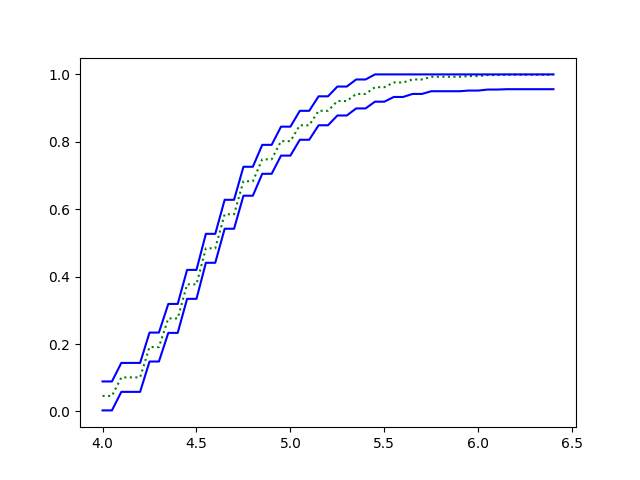
\includegraphics[width=0.6\textwidth]{7-Estimating_the_CDF_and_Statistical_Functionals/Ex7_7.png}
			\end{center}
		\end{itemize}
	\item Get the data on eruption times and waiting times between eruptions of the Old Faithful geyser from the website. Estimate the mean waiting time and give a  error for the estimate. Also, give a 90 percent confidence interval for the mean waiting time. Now estimate the median waiting time. In the next chapter we will see how to get the standard error for the median.
		\begin{itemize}
			\item \texttt{https://www.stat.cmu.edu/~larry/all-of-statistics/=data/faithful.dat}
			\item I modified the text file, removing the text above the table before importing it.
			\item
				\begin{minted}{python}
import numpy as np
import pandas as pd
import scipy

file_path = "Data/faithful.dat"

column_names = ['eruptions', 'waiting']
df = pd.DataFrame(columns=column_names)

with open(file_path, 'r') as file:
    next(file)  # Skips the header row
    for line in file:
        _, eruptions, waiting = line.strip().split()
        data_dict = {'eruptions': float(eruptions), 'waiting': int(waiting)}
        df = df.append(data_dict, ignore_index=True)


X = df["waiting"].values
n = len(X)
mu = np.mean(X)
variance = np.dot(X - mu, X - mu) / (2 * n)
sigma = np.sqrt(variance)

print(f"mu = {mu:.2f}\nse = {sigma:.2f}")

z = scipy.stats.norm.ppf(0.95)
print(f"(mu-z*se, mu+z*se) = ({mu - z * sigma:.2f}, {mu + z * sigma:.2f})")
				\end{minted}
		\end{itemize}
	\item $100$ people are given a standard antibiotic to treat an infection and another $100$ are given a new antibiotic. In the first group, $90$ people recover; in the second group, $85$ people recover. Let $p_1$ be the probability of recovery under the standard treatment and let P2 be the probability of recovery under the new treatment. We are interested in estimating $\theta = p_1 - p_2$. Provide an estimate, standard error, an $80$ percent confidence interval, and a $95$ percent confidence interval for $B$.
	\item 
\end{enumerate}

\subsection{The Bootstrap}
\begin{enumerate}
	\item Consider the data in Example 8.6. Find the plug-in estimate of the correlation coefficient. Estimate the standard error using the bootstrap. Find a 95 percent confidence interval using the Normal, pivotal, and percentile methods.
	\item (Computer Experiment.) Conduct a simulation to compare the various bootstrap confidence interval methods. Let $n = 50$ and let $T(F) = \int(x - \mu)^3 dF(x)/\sigma^3$ be the skewness. Draw $Y_1, \dots, Y_n \sim \mathcal{N}(O,1)$ and set $X_i = e^{Y_i}, i = 1, \dots, n$. Construct the three types of bootstrap $95$ percent intervals for $T(F)$ from the data $X_1, \dots, X_n$. Repeat this whole thing many times and estimate the true coverage of the three intervals.
	\item Let
	$$
	X_1, \dots, X_n \sim t_3
	$$
	where $n = 25$. Let $\theta = T(F) = (q_{.75} - q_{.25}) / 1.34$ where $q_p$ denotes the $p$th quantile. Do a simulation to compare the coverage and the length of the following confidence intervals for $\theta$: (i) Normal interval with standard error from the bootstrap, (ii) bootstrap percentile interval, and (iii) pivotal bootstrap interval.
	\item Let $X_1, \dots, X_n$ be distinct observations (no ties). Show that there are
	$$
	\binom{2n - 1}{n}
	$$
	distinct bootstrap samples.

	Hint: Imagine putting $n$ balls into $n$ buckets.
	\item Let $X_1, \dots, X_n$ be distinct observations (no ties). Let $X_1^*, \dots, X_n^*$ denote a bootstrap sample and let
	$$
	\overline{X}_n^* = \frac{1}{n} \sum_{i = 1}^n X_i^*.
	$$
	Find: $E(\overline{X}_n^* | X_1, \dots, X_n), V(\overline{X}_n^*|X_1, \dots, X_n), E(\overline{X}_n^*)$ and $V(\overline{X}_n^*)$.
	\item (Computer Experiment.) Let $X_1, \dots, X_n \sim \mathcal{N}(\mu, 1)$. let $\theta = e^\mu$ and let $\hat{\theta} = e^{\overline{X}}$. Create a data set (using $\mu = 5$) consisting of $n = 100$ observations.
		\begin{enumerate}
			\item Use the bootstrap to get the $\se$ and $95\%$ confidence interval for $\theta$.
			\item Plot a histogram of the bootstrap replications. This is an estimate of the distribution of $\hat{\theta}$. Compare this to teh true sampling distribution of $\hat{\theta}$.
		\end{enumerate}
	\item Let $X_1, \dots, X_n \sim U(0, \theta)$. Let $\hat{\theta} = X_{\max} = \max\{X_1, \dots, X_n\}$. Generate a data set of size $50$ with $\theta = 1$.
		\begin{enumerate}
			\item Find the distribution of $\hat{\theta}$. Compare the true distribution of $\hat{\theta}$ to the histograms from the bootstrap.
			\item This is a case where the bootstrap does very poorly. In fact, we can prove that this is the case. Show thatt $P(\hat{\theta} = \hat{\theta}) = 0$ and yet $P(\hat{\theta}^* = \hat{\theta}) = 0.632.$ Hint: show that,
			$$
			P(\hat{\theta}^* = \hat{\theta}) = 1 - (1 - (1 / n))^n
			$$
			and then tkae the limit as $n$ gets large.
		\end{enumerate}
	\item Let $T_n = \overline{X}_n^2, \mu = E(X_1),$
	$$
	\alpha_k = \int |x - \mu|^k dF(x)
	$$
	and
	$$
	\hat{\alpha}_k = \frac{1}{n} \sum_{i = 1}^n |X_i - \overline{X}_n|^k.
	$$
	Show that
	$$
	v_{\operatorname{boot}} = \frac{4 \overline{X}_n^2 \hat{\alpha}_2}{n} + \frac{4 \overline{X}_n \hat{\alpha}_3}{n^2} + \frac{\hat{\alpha}_4}{n^3}.
	$$
\end{enumerate}

\subsection{Parametric Inference}

\subsection{Hypothesis Testing and p-values}

\subsection{Bayesian Inference}

\subsection{Statistical Decision Theory}

\section{Statistical Models and Methods}
\subsection{Linear and Logistic Regression}
\begin{enumerate}
	\item Prove Theorem 13.4.
	\item Prove the formulas for the standard errors in Theorem 13.8. You should regard the $X_i$ as fixed constants.
	\item Consider the regression through the origin model:
	$$
	Y_i = \beta X_i + \varepsilon.
	$$
	Find the least squares estimate for $\beta$. Find the standard error of the estimate. Find conditions that guarantee that the estimate is consistent.
	\item Prove equation (13.25)
	\item In the simple linear regression model, construct a Wald test for $H_0 : \beta_1 = 17\beta_0$ versus $H_1 : \beta_1 \neq 17\beta_0$.
	\item Get the passenger car mileage data from
	
	\texttt{http://lib.stat.cmu.ed u/DASL /Datafiles/ carmpgdat.html}
		\begin{enumerate}
			\item Fit a simple linear regression model to predict $\operatorname{MPG}$ (miles per gallon) from $\operatorname{HP}$ (horsepower). Summarize your analysis including a plot of the data with the fitted line.
				\begin{itemize}
				\item
				\begin{minted}{python}
import numpy as np
import pandas as pd
import matplotlib.pyplot as plt

def plotLine(x, y, color = "green", linestyle = "dotted"):
    plt.plot(x, y, color = color, linestyle = linestyle)

file_path = "Data/carmileage.dat"
column_names = ["Vol", "HP", "MPG", "SP", "WT"]
df = pd.read_csv(file_path,
                 sep='\t',
                 header=None,
                 names=column_names,
                 skiprows=1,
                 usecols=[1, 2, 3, 4, 5])

X, Y = df["HP"], df["MPG"]
n = len(X)

mu_X = np.mean(X)
mu_Y = np.mean(Y)

offsetNorm = np.dot(X - mu_X, X - mu_X)

beta1 = np.dot(X - mu_X, Y - mu_Y) / offsetNorm
beta0 = mu_Y - beta1 * mu_X

lineFunc = lambda x : beta0 + beta1 * x
x, y = [40, 350], [lineFunc(40), lineFunc(350)]

rss = np.dot(Y - lineFunc(X), Y - lineFunc(X))
var = rss / (len(X) - 2)
sigma = np.sqrt(var)

plt.scatter(X, Y)

plotLine(x, y, color = "red", linestyle = "-")

plotLine(x, y - sigma)
plotLine(x, y + sigma)
plotLine(x, y - 2 * sigma)
plotLine(x, y + 2 * sigma)

plt.xlabel("Horsepower")
plt.ylabel("Miles per gallon")

plt.savefig("Ex13_6.png")

plt.show()
				\end{minted}
					\begin{center}
					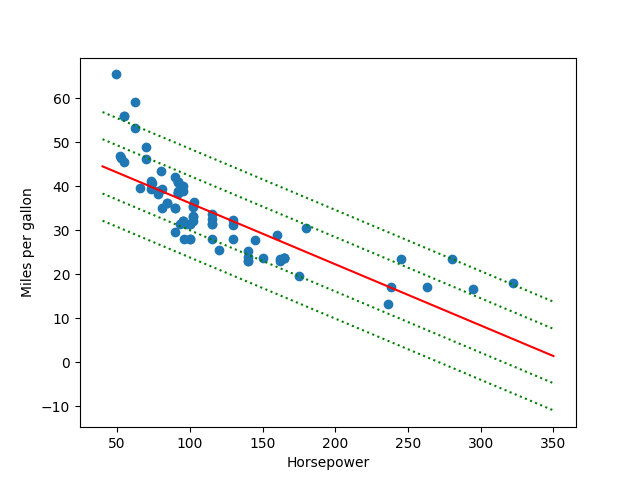
\includegraphics[width=0.6\textwidth]{13-Linear_And_Logistic_Regression/Ex13_6.png}
					\end{center}
				\end{itemize}
			\item Repeat the analysis the use $\log(\operatorname{MPG})$ as the response. Compare the analyses.
		\end{enumerate}
	\item Get the passenger car mileage data from

	\texttt{http://lib.stat.cmu.edu/DASL/Datafiles/carmpgdat.html}
		\begin{enumerate}
			\item Fit a multiple linear regression model to predict $\operatorname{MPG}$ (miles per gallon) from the other variables. Summarize your analysis.
			\item Use Mallow $C_p$ to select a best sub-model. To search through the models try (i) forward stepwise, (ii) backward stepwise. Summarize your findings.
			\item Use the Zheng-Loh model selection method and compare to (b).
			\item Perform all possible regressions. Compare $C_p$ and $\operatorname{BIC}$. Compare the results.
		\end{enumerate}
	\item Assume a linear regression model with Normal errors. Take $\sigma$ known. Show that the model with highest $\operatorname{AIC}$ (equation (13.27)) is the model with the lowest Mallows $C_p$ statistic.
	\item 
	\item In this question we take a closer look at prediction intervals. Let
	$$
	\theta = \beta_0 + \beta_1 X_*,
	$$
	and let
	$$
	\hat{\theta} = \hat{\beta}_0 + \hat{\beta}_1 X_*.
	$$
	Thus, $\hat{Y}_* = \hat{\theta}$ while $Y_* = \theta + \varepsilon$. Now, $\hat{\theta} \approx \mathcal{N}(\theta, \se^2)$, where
	$$
	\se^2 = V(\hat{\theta}) = V(\hat{beta}_0 + \hat{\beta}_1 x_*).
	$$
	Note that $V(\hat{\theta})$ is the same as $V(\hat{Y}_*)$. Now, $\hat{\theta} \pm 2 \sqrt{V(\hat{\theta})}$ is an approximate $95\%$ percent confidence interval for $\theta = \beta_0 + \beta_1 + x_*$ using the usual argument for a confidence interval. But, as you shall now show, it is not a valid confidence interval for $Y_*$.
		\begin{enumerate}
			\item Let $s = \sqrt{V(\hat{Y}_*)}$. Show that
			$$
			\begin{aligned}
			P(\hat{Y}_* - 2s < Y_* < \hat{Y}_* + 2 s) &\approx P\left( -2 < \mathcal{N}\left(0, 1 + \frac{\sigma^2}{s^2}\right) < 2\right) \\
			&\neq 0.95.
			\end{aligned}
			$$
			\item The problem is that the quantity of interest $Y_*$ is equal to a paramter $\theta$ plus a random variable. We can fix this by defining
			$$
			\xi_n^2 = V(\hat{Y}_*) + \sigma^2 = \left(\frac{\sum_i (x_i - x_*)^2}{n \sum_i (x_i - \overline{x})} + 1\right)\sigma^2.
			$$
			In practice, we can substitute $\hat{\sigma}$ for $\sigma$ and we denote the resulting quantity by $\hat{\xi}_n$. Now consider the interval $\hat{Y}_* \pm 2 \hat{\xi}_n$. Show that
			$$
			P(\hat{Y}_* - 2\hat{\xi}_n < Y_* < \hat{Y}_* + 2 \hat{\xi}_n) \approx P(-2 < \mathcal{N}(0, 1) < 2) \approx 0.95.
			$$
		\end{enumerate}
	\item Get the Coronary Risk-Factor Study (CORIS) data from the book web site. Use backward stepwise logistic regression based on AIC to select a model. Summarize your results.
\end{enumerate}

\subsection{Multivariate Models}
\begin{enumerate}
	\item Prove Theorem 14.1
	\item Find the Fisher information matrix for the $\MLE$ of a Multinomial.
	\item (Computer Experiment.) Write a function to generate nsim observations from a $\operatorname{Multinomial}(n, p)$ distribution.
	\item (Computer Experiment.) Write a function to generate $\operatorname{nsim}$ observations from a Multivariate normal with given mean $\mu$ and covariance matrix $\Sigma$.
	\item (Computer Experiment.) Generate $100$ random vectors from a $\mathcal{N}(\mu, \Sigma)$ distribution where
	$$
	\begin{aligned}
	\mu = \begin{pmatrix} 3 \\ 8 \end{pmatrix},&&
	\Sigma = \begin{pmatrix}
	1 & 1 \\
	1 & 2
	\end{pmatrix}.
	\end{aligned}
	$$
	Plot the simulation as a scatterplot. Estimate the mean and covariance matrix $\Sigma$. Find the correlation $\rho$ between $X_1$ and $X_2$. Comapre this with the sample correlations from your simulation. Find $95\%$ confidence interval for $\rho$. Use two methods: the bootstrap and Fisher's method. Compare.
	\item (Computer Experiment.) Repeat the previous exercise $1000$ times. Compare teh coverage of the two confidence intervals for $\rho$.
\end{enumerate}

\subsection{Inference About Independence}
\begin{enumerate}
	\item Prove Theorem 15.2.
	\item Prove Theorem 15.3.
	\item Prove Theorem 15.6.
	\item The New York Times (January 8, 2003, page A12) reported the following data on death sentencing and race, from a study of Maryland:
	\begin{center}
		\begin{tabular}{|c|c|c|}
			\hline
			& Black Victim & White Victim \\
			\hline
			Death Sentence & 14 & 62 \\
			\hline
			No Death Sentence & 641 & 594 \\
			\hline
		\end{tabular}
	\end{center}
	Analyze the data using the tools from this chapter. Interpret the results. Explain why, based only on this information, you can't make causal conclusions. (The authors ofthe study did use much more information in their full report.)
	\item Anaylsis teh data on the variables Age and Financial Status from:
	\texttt{http://lib.stat.cmu.edu/DASL/Datafiles/montanadat.html}
	\item Estimate the correlation between temperature and latitude using the data from
	\texttt{http://lib.stat.cmu.edu/DASL/Datafiles/USTemperatures.html}
	Use the correlation coefficient. Provide estimates, tests, and confidence intervals.
	\item Test whether calcium intake and drop in blood pressure are associated. Use the data in
	\texttt{http://lib.stat.cmu.edu/DASL/Datafiles/Calcium.html}
\end{enumerate}

\subsection{Causal Inference}
\begin{enumerate}
	\item Create an example like Example 16.2 in which $\alpha > 0$ and $\theta < 0$.
	\item Prove Theorem 16.4.
	\item Suppose your are given data $(X_i, Y_i), 1 \leq i \leq n$ from an observational study, where $X_i, Y_1 \in \{0, 1\}$. Although it is not possible to estimate the causal effect $\theta$, it is possible to put bounds on $\theta$. Find upper and lower bounds on $\theta$ that can be consistently estimated from the data. Show that the bounds have width $1$.
	Hint: Note that
	$$
	E(C_1) = E(C_1|X = 1)P(X = 1) + E(C_1|X = 0)P(X = 0).
	$$
	\item Suppose that $X \in \mathbb{R}$ and that, for each subject $i$, $C_i(x) = \beta_{1i}x$. Each subject has their own slope $\beta_{1i}$. Construct a joint distribution on $(\beta_1, X)$ such that $P(\beta_1 > 0) = 1$ but $E(Y|X = x)$ is a decreasing function on $x$, where  $Y = C(X)$. Interpret.
	\item Let $X \in \{0, 1\}$ be a binary treatment variable and let $(C_0, C_1)$ denote the correspondingg potential outcomes. Let $Y = C_X$ denote the observed response. Let $F_0$ and $F_1$ be cumulative distribution functions for $C_0$ and $C_1$. Assume that $F_0$ and $F_1$ are both continuous and strictly increasing. Let $\theta = m_1 - m_0$ where $m_i = F_i^{-1}(1 / 2)$ is the median of $C_i, i = 0, 1$. Suppose that the treatment $X$ is assigned randomly. Find an expression for $\theta$ involving only the joint distribution of $X$ and $Y$.
\end{enumerate}

\subsection{Directed Graphs and Conditional Independence}

\subsection{Undirected Graphs}

\subsection{Log-Linear Models}

\subsection{Nonparametric Curve Estimation}

\subsection{Smoothin Using Orthogonal Functions}

\subsection{Classification}

\subsection{Probability Redux: Stochastic Processes}

\subsection{Simulation Methods}

\end{document}